\documentclass[11pt, a4paper, oneside]{Thesis}
\graphicspath{{figures/}}
\DeclareGraphicsExtensions{.pdf,.jpeg,.png,.jpg}
\usepackage[square, numbers, comma, sort,super]{natbib}
\usepackage{titlesec}
\usepackage{float}
\usepackage{hyperref}
\usepackage[nopostdot,nonumberlist,acronym,toc,section,xindy]{glossaries}

 
\makenoidxglossaries
 
 \newglossaryentry{anaphylaxis}
{
       name=Anaphylaxis,
       description={A severe, potentially life-threatening allergic reaction that can develop rapidly.}
}

\newglossaryentry{angiography}
{
       name=Angiography,
       description={An imaging technique used to visualise the inside of blood vessels and organs, and particularly the visualisation of the veins and arteries supplying a given organ.}
}

\newglossaryentry{aperture}
{
        name=Aperture,
        description={An opening through which light can travel.}
}

\newglossaryentry{astigmatism}
{
        name=Astigmatism,
     description={A common and usually minor eye condition that causes blurred or distorted vision.}
}

\newglossaryentry{atrophy}
{
        name=Atrophy,
        description={A partial or complete wasting of a part of the body.}
}

\newglossaryentry{bipolar_cell}
{
        name=Bipolar cell,
       description={Part of the retina, bipolar cells are located between the photoreceptors and ganglion cells.  They act to transmit signals between the two.}
}

\newglossaryentry{chromatic_aberration}
{
        name=Chromatic aberration,
        description={A type of distortion where the lens fails to focus all colours to the same convergence point. This manifests itself as fringes of colour along the boundaries that separate the light and dark parts of an image.}
}

\newglossaryentry{cornea}
{
        name=Cornea,
      description={The transparent front part of the eye covering the pupil, iris and anterior chamber.}
}

\newglossaryentry{emmetropic}
{
        name=Emmetropic,
        description={Describes the state of vision wherein an object at infinity is in sharp focus, with the eye lens in a relaxed state.  This is achieved in the normal eye when the refractive power of the cornea and the axial length of the eye balance out.}
}

\newglossaryentry{epithelium}
{
        name=Epithelium,
        description={Is one of the four basic types of animal tissue, along with connective tissue, muscle tissue and nervous tissue. Epithelial tissues line the cavities and surfaces of structures throughout the body.}
}

\newglossaryentry{fluorescein}
{
        name=Fluorescein,
        description={A synthetic organic compound that is commonly used as a fluorescent tracer in microscopy and medical imaging.}
}

\newglossaryentry{fovea_centralis}
{
        name=Fovea centralis,
        description={A small pit composed of closely packed cone cells that is located in the macula of the eye.  Responsible for producing sharp central vision.}
}

\newglossaryentry{fundus}
{
        name=Fundus,
        description={The interior surface of the eye, including structures such as the retina, optic disc, macula and fovea.}
}

\newglossaryentry{ganglion_cell}
{
        name=Ganglion cell,
        description={A type of neuron that is located near the inner surface of the retina.  It receives visual information from the photoreceptors via bipolar cells.}
}

\newglossaryentry{hyperopia}
{
        name=Hyperopia,
        description={Commonly known as being long sighted, it is a vision defect that can cause difficulty in focusing on nearby objects.}
}

\newglossaryentry{hyperspectral_imaging}
{
        name=Hyperspectral Imaging,
        description={Processes information from across the electromagnetic spectrum.  Obtains
        the spectrum for each pixel in the image of a scene, with the purpose of finding objects or
         detecting processes.}
}

\newglossaryentry{interferometry}
{
name=Interferometry,
description={A collection of techniques in which electromagnetic waves are superimposed in order to extract more information about the waves.}
}

\newglossaryentry{intraocular}
{
        name=Intraocular,
        description={Inside of the eye.}
}

\newglossaryentry{isotropy}
{
        name=Isotropy,
        description={Uniformity in all orientations.}
}

\newglossaryentry{leukocytes}
{
        name=Leukocytes,
        description={White blood cells.}
}

\newglossaryentry{lipofuscin}
{
name=Lipofuscin,
    	description={The name given to pigment granules composed of lipid-containing residues of lysosomal digestion.  Considered to be one of the aging pigments, and commonly found in the retina and in ganglion cells, as well as other organs such as the liver and kidney.}
}

\newglossaryentry{macula}
{
        name=Macula,
        description={An oval-shaped pigmented area near the center of the retina.}
}

\newglossaryentry{macular_edema}
{
        name=Macular Edema,
        description={An accumulation of fluid within the retina at the macular area, causing the macula to thicken and swell.}
}

\newglossaryentry{microaneurysm}
{
name=Microaneurysm,
description={A retinal microaneurysm is a small area of blood protruding from a blood vessel in the back of the eye.  Can lead to blood leaking into the surrounding retinal tissue.}
}
 
\newglossaryentry{mydriasis}
{
name=Mydriasis,
description={Dilation of the pupil of the eye.}
}

\newglossaryentry{myopia}
{
name=Myopia,
description={A condition of the eye where the light that comes in does not directly focus on the retina but in front of it, causing the image that one sees when looking at a distant object to be out of focus, but in focus when looking at a close object.}
}

\newglossaryentry{neovascular}
{
name=Neovascular,
description={Describes the proliferation of blood vessels in tissue that does not normally contain them.}
}

\newglossaryentry{oblate}
{
	name=Oblate,
	description={The distortion of a sphere having an equatorial diameter greater than the distance between poles; compressed along or flattened at the poles.}
}

\newglossaryentry{oximetry}
{
	name=Oximetry,
	description={A procedure that measures the amount of oxygen in the blood.}
}

\newglossaryentry{papilledema}
{
	name=Papilledema,
description={Optic disc swelling that is usually caused by increased intracranial pressure.}
}

\newglossaryentry{pathology}
{
	name=Pathology,
description={A branch of medical science primarily concerning the examination of organs, tissues, and bodily fluids in order to make a diagnosis of disease.}
}

\newglossaryentry{phenotype}
{
	name=Phenotype,
	description={The composite of an organism's characteristics, such as its morphology, biochemical and physiological properties.  Dependent on which genes are dominant and on the interaction between expressed genes and the environment.}
}

\newglossaryentry{photoreceptors}
{
name=Photoreceptors,
description={Can be divided into rod cells and cone cells.  Specialised types of neurons found in the retina.  Convert light into signals that can stimulate biological processes by absorbing photons that trigger a change in the cell?s membrane potential.}
}

\newglossaryentry{presbyopia}
{
	name=Presbyopia,
	description={A condition associated with aging in which the eye exhibits a progressively diminished ability to focus on near objects.}
}

\newglossaryentry{prolate}
{
	name=Prolate,
	description={The distortion of a sphere having the distance between the poles longer than the equatorial diameter.}
}

\newglossaryentry{red_reflex}
{
name=Red reflex,
description={Refers to the red reflection of light from the eye's retina that can be observed when using an ophthalmoscope.}
}

\newglossaryentry{retina}
{
        name=Retina,
        description={A light-sensitive layer of tissue that lines the inner surface of the eye.
        The optics of the eye create an image on the retina, serving much the same function
        as the film in a camera.}
}

\newglossaryentry{retinopathy}
{
        name=Retinopathy,
        description={Persistent or acute damage to the retina.  A common manifestation of systemic diseases such as diabetes and high blood pressure.}
}

\newglossaryentry{sclera}
{
        name=Sclera,
        description={Commonly known as the white of the eye.  It is an opaque, protective layer of the eye containing collagen and elastic fibre.}
}

\newglossaryentry{scleral_venous_sinus}
{
        name=Scleral venous sinus,
        description={Also known as Schlemm?s canal.  It is a channel that collects fluid from the anterior chamber of the eye and delivers it into the bloodstream via the anterior ciliary veins.}
}

\newglossaryentry{tomographic_imaging}
{
        name=Tomographic imaging,
        description={Imaging by sectioning, through the use of a penetrating wave.}
}

\newglossaryentry{trachoma}
{
	name=Trachoma,
	description={A type of bacterial eye infection, and the leading cause of preventable blindness in the world.}
}

\newglossaryentry{vitreoretinal}
{
        name=Vitreoretinal,
        description={Relating to the vitreous body and the retina.}
}

\newglossaryentry{vitreuous_humour}
{
        name=Vitreous humour,
        description={The transparent tissue filling the eyeball behind the lens.}
}
 
\newacronym{amd}{AMD}{Age Related Macular Degeneration}
\newacronym{oct}{OCT}{Optical Coherence Tomography}
\newacronym{cslo}{cSLO}{Confocal Scanning Laser Ophthalmoscope}
\newacronym{rpe}{RPE}{Retinal Pigment Epithelium}
\newacronym{sift}{SIFT}{Scale Invariant Feature Transform}
\newacronym{led}{LED}{Light Emitting Diode}
\newacronym{laser}{LASER}{Light Amplification by Stimulated Emission of Radiation}
\newacronym{sled}{SLED}{Super-luminescent Light Emitting Diode}
\newacronym{sld}{SLD}{Super-luminescent Light Emitting Diode}
\newacronym{tdoct}{TD-OCT}{Time Domain Optical Coherence Tomography}
\newacronym{fdoct}{FD-OCT}{Fourier Domain Optical Coherence Tomography}
\newacronym{sdoct}{FD-OCT}{Spectral Domain Optical Coherence Tomography}
\newacronym{cad}{CAD}{Computer Aided Diagnosis}
\newacronym{ccd}{CCD}{Charge Coupled Device}
\newacronym{cmos}{CMOS}{Complementary Metal Oxide Semiconductor}
\newacronym{dme}{DME}{Diabetic Macular Edema}
\newacronym{seads}{SEADs}{Symptomatic Exudate-Associated Derangements}
\newacronym{nco}{NCO}{Neural Canal Opening}
\newacronym{ao}{AO}{Adaptive Optics}
\newacronym{faf}{FAF}{Fundus Auto-Fluorescence}

\titleformat{\chapter}[display]
  {\normalfont\huge\bfseries}{}{0pt}{\huge}
\titleformat{name=\chapter,numberless}[display]
  {\normalfont \huge\bfseries}{}{0pt}{\huge}

\title{\ttitle} 

\begin{document}
\frontmatter % Page umbering style i, ii, iii, iv...for the pre-content pages
\setstretch{1.3} % Line spacing
\fancyhead{} % Clears all page headers and footers
\rhead{\thepage} % Sets the right side header to show the page number
\lhead{} % Clears the left side page header
\pagestyle{fancy}
\newcommand{\HRule}{\rule{\linewidth}{0.5mm}} % Put lines on the title page

% PDF meta-data
\hypersetup{pdftitle={\ttitle}}
\hypersetup{pdfauthor={\authornames}}


%-------------------------------------------------------------------------------
% TITLE PAGE
%-------------------------------------------------------------------------------

\begin{titlepage}
\begin{center}

\textsc{\LARGE The University of Edinburgh}\\[1.5cm]
\HRule \\[0.8cm] % Horizontal line

\textsc{\huge \ttitle }\\[0.2cm]
\HRule \\[0.5cm] % Horizontal line
\textsc{\Large \deptname}\\[1.0cm]

\large \today \\[1cm]


\includegraphics[width=4.0cm]{logo}\\[1cm]

\textsc{\small By Magdalen Berns, Eskil Joergensen, Calum Macewen, Morgan Shaner and Matt Toman} \\[1cm]

\textsc{\Large{Abstract}}\\
\end{center}

In order to explore the challenges ophthalmologists have to overcome when making
accurate diagnoses by examination of the complex optical system that is the human eye,
an extensive investigation into technology that underpins retinal imaging is required.
Many diseases manifest themselves in the retina, therefore it is vital to determine ways
to view and image this tissue. This review has focused on advances in the three main
devices which are used in retinal imaging research: the fundus camera, the \Gls{cslo}
and \Gls{oct}. A detailed introductionto the eye along with its dysfunction, pathology and
injury is provided, in addition, a comprehensive overview of the early origins of
ophthalmoscopy in the 19th century is given. The analysis concludes with a discussion
about future research in this area of research, covering the most recent advancements
in imaging industrial science which utilise adaptive optics and two-photon microscopy.
\end{titlepage}


%-------------------------------------------------------------------------------
% ACKNOWLEDGEMENTS
%-------------------------------------------------------------------------------

\acknowledgements{\addtocontents{toc}{\vspace{1em}}
Prof. Caroline Macewen - Consultant Ophthalmologist Ninewells Hospital,
Editor Eye-Nature, Senior Vice President Royal College of Ophthalmologists

Pauline MacEwen - Optometrist, Independent Prescriber, Retinal Screening Specialist

Dr. William Hossack - Team Advisor

Jano van Hemert - Optos Academic Liaison, Head of Imaging

}

\clearpage % Start a new page
 
%-------------------------------------------------------------------------------
% CONTENTS
%-------------------------------------------------------------------------------
\pagestyle{fancy}

\lhead{\emph{Contents}} % Set the left side page header to "Contents"
\tableofcontents % Write out the Table of Contents

\clearpage % Start a new page


%-------------------------------------------------------------------------------
% CONTENT CHAPTERS
%-------------------------------------------------------------------------------
\mainmatter % Numeric (1,2,3...) page numbering
\pagestyle{fancy}
\chapter{Introduction}

\label{intro}
\lhead{\emph{Introduction}}

There are many diseases that manifest themselves  in the  retina, thus
for many years scientists have made producing a detailed image of the
retina their life's work.  Although the primary  purpose of this technology
is for diagnostic and monitoring purposes, ophthalmologists are using
these devices to study the retina's structure to gain insight into the
manifestations of these diseases.  There are many physical principles
behind the technology used to image the retina; including understanding
the complex optics of the eye, utilising the optics of the eye to obtain an
image of the retina and the use of physically advanced systems to gain
insight into the retinal structure.

This review focuses on three main technologies in retinal 
imaging research: fundus cameras, \Gls{cslo} and \Gls{oct}.
To introduce these technologies a detailed introduction 
to the eye and its dysfunction, pathology, and injury is provided 
along with a comprehensive overview of the early origins of 
ophthalmoscopy in the 19th century.  To highlight the shortcomings 
of the current state of these technologies, there is a section discussing 
the future research following the discussion on fundus imaging and 
optical coherence tomography.  This discussion covers the 
most recent advancements in imaging technology utilising adaptive 
optics and two-photon microscopy.  The purpose of this review is to 
introduce a complex optical system and provide an extensive 
investigation into the technology that underpins retinal imaging.

% Author: Magdalen Berns

\chapter{The Physiology of The Eye}

\label{anatomy}
\lhead{\emph{The Physiology of The Eye}}
\section{A Normal, Healthy Eye}

The human eye has many members which combine to allow human beings to
interpret the visual light into a continuum of recognisable imagery
to more easily identify and interact with surroundings. \Fref{fig:eye_simple}
shows a simple schematic diagram of the layout of the eye.

\begin{figure}[!htbp]
  \centering
    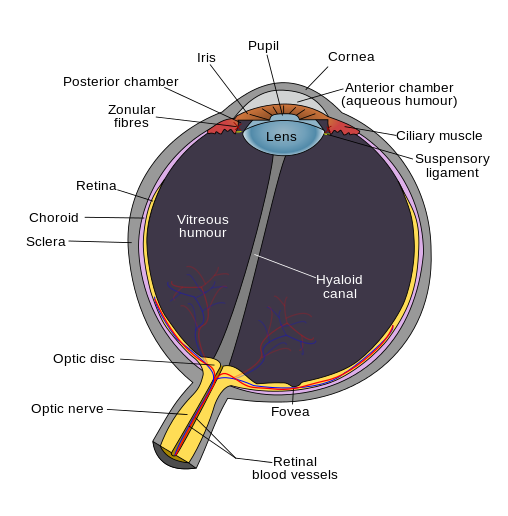
\includegraphics{figures/schematic_diagram_of_the_human_eye}
  \caption{A simple schematic diagram of the layout of the eye.\cite{wikiRhcastilhos}}
  \label{fig:eye_simple}
\end{figure}

The cornea of the eye is a transparent layer around 0.6mm thick
which curves around the iris of the eye as well as its anterior
chamber.\cite{yaylali1997corneal,thoft1983x,patel1994refractive}
With a mean refractive index of around 1.4 (about the same as water),
the cornea allows plenty of light to pass through, but refracts as a
convergent lens due to its convex, shape. \Eref{eq:refractive} shows
Snell's Law of refraction for a light wave passing through two
different isotropic materials which have refractive indices $n_1$
and $n_2$, respectively.

\begin{figure}[htbp]
  \centering
    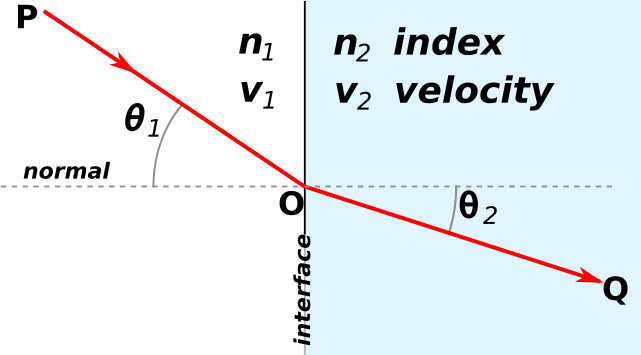
\includegraphics{figures/snells}
  \caption{Snell's law for diffraction at an interface where $n_1$ \textless $n_2$.\cite{wikisnell}}
  \label{fig:snell}
\end{figure}

The angle $\theta_1$ is normal to the boundary between $n_1$ and $n_2$
and the angle $\theta_2$ is normal to the boundary between $n_2$ and $n_1$
as shown in \fref{fig:snell}

\begin{equation}
n_1\sin\theta_1=n_2\sin\theta_2
\label{eq:refractive}
\end{equation}

The radius of the human cornea tends to decrease with age and the cornea
itself, takes on a more spherical shape.\cite{guirao2000optical} Its
outermost surface is made of epithelial cells which are continuously lost
and replaced.\cite{jester1999cellular,hassell2010molecular} The reproduction
of cells is facilitated in part by tear ducts, which  serve to moisten the
eyes and remove harmful bacteria.\cite{holly1977tear}

There is a small circular opening in the iris, (the coloured section of
the eye) the pupil, has an aperture which dilates to allow an appropriate
amount of refracted light to pass through the lens. Light is refracted
once again through the lens converges towards a focal point on the back
of the eye. The lens makers expression in \eref{eq:lens_makers} is an
expression described by the diagram in \fref{fig:convergent_lens} which
shows light passing through a convex lens for calculating the focal point,
$f$ of distances $S_1$ and $S_2$ either side of a given convex lens.
\cite{greivenkamp2004field}

\begin{equation}
\frac{1}{S_1} + \frac{1}{S_2} = \frac{1}{f}
\label{eq:lens_makers}
\end{equation}

\begin{figure}[htbp]
  \centering
    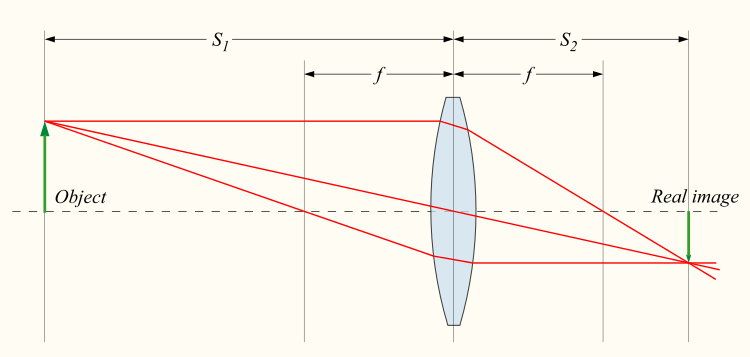
\includegraphics{figures/convergent_lens2}
  \caption{light passing through a convex lens for calculating the focal
  point, $f$ of distances $S_1$ and $S_2$ either side of a given convex lens.}
  \label{fig:convergent_lens}
\end{figure}

A ciliary body of tissue made up of fiber and muscle which accommodates the
lens and secretes a fluid, known as Aqueous Humour into a canal that flows
around the circumference of the eye called the Scleral Venous Sinus.
\cite{bill1970effects,dvorak1934schlemm}

When it becomes necessary to focus on objects at short distances, the
ciliary body muscles contract and suspensory ligaments attached to the
posterior chamber and the posterior lens to become taut, causing the
lens to become somewhat flatter, in response to applied contractile
forces. When objects are far away the light is more parallel to the lens'
principle axis, the muscles relax and suspensory ligaments attached to
the posterior chamber and the posterior lens so that it is no longer being
accommodated so it can take on a more rounded shape.

Photons of light are refracted out of the lens, before they pass through
a clear substance called the vitreous chamber and land onto the retina,
which is also transparent. A diagram indicating the optic axis and
visual axis is shown in \fref{fig:optic_axis}.

\begin{figure}[htbp]
  \centering
    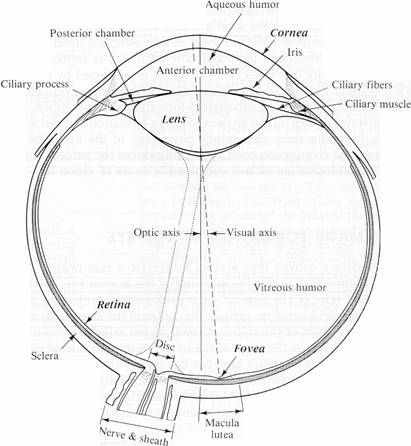
\includegraphics{figures/eye_diagram}
  \caption{A diagram of the eye showing of the visual
   and optic axis, the cornea, the retina and the fovea}
  \label{fig:optic_axis}
\end{figure} 

The retina is a membrane which covers the entire receptive field of
vision, it is part of the central nervous system.\cite{rogers1983neurite}
Just behind the retina are ganglion cells, biploar cells, cones and rods.
These are supported by pigment epithelium cells and the choroid, a vascular
bed of tissues which supply the retina with blood and removes toxins.
\cite{lutty1996localization} A schematic overview of the core retinal
constitution is given in \fref{fig:retina}

\begin{figure}[htbp]
  \centering
    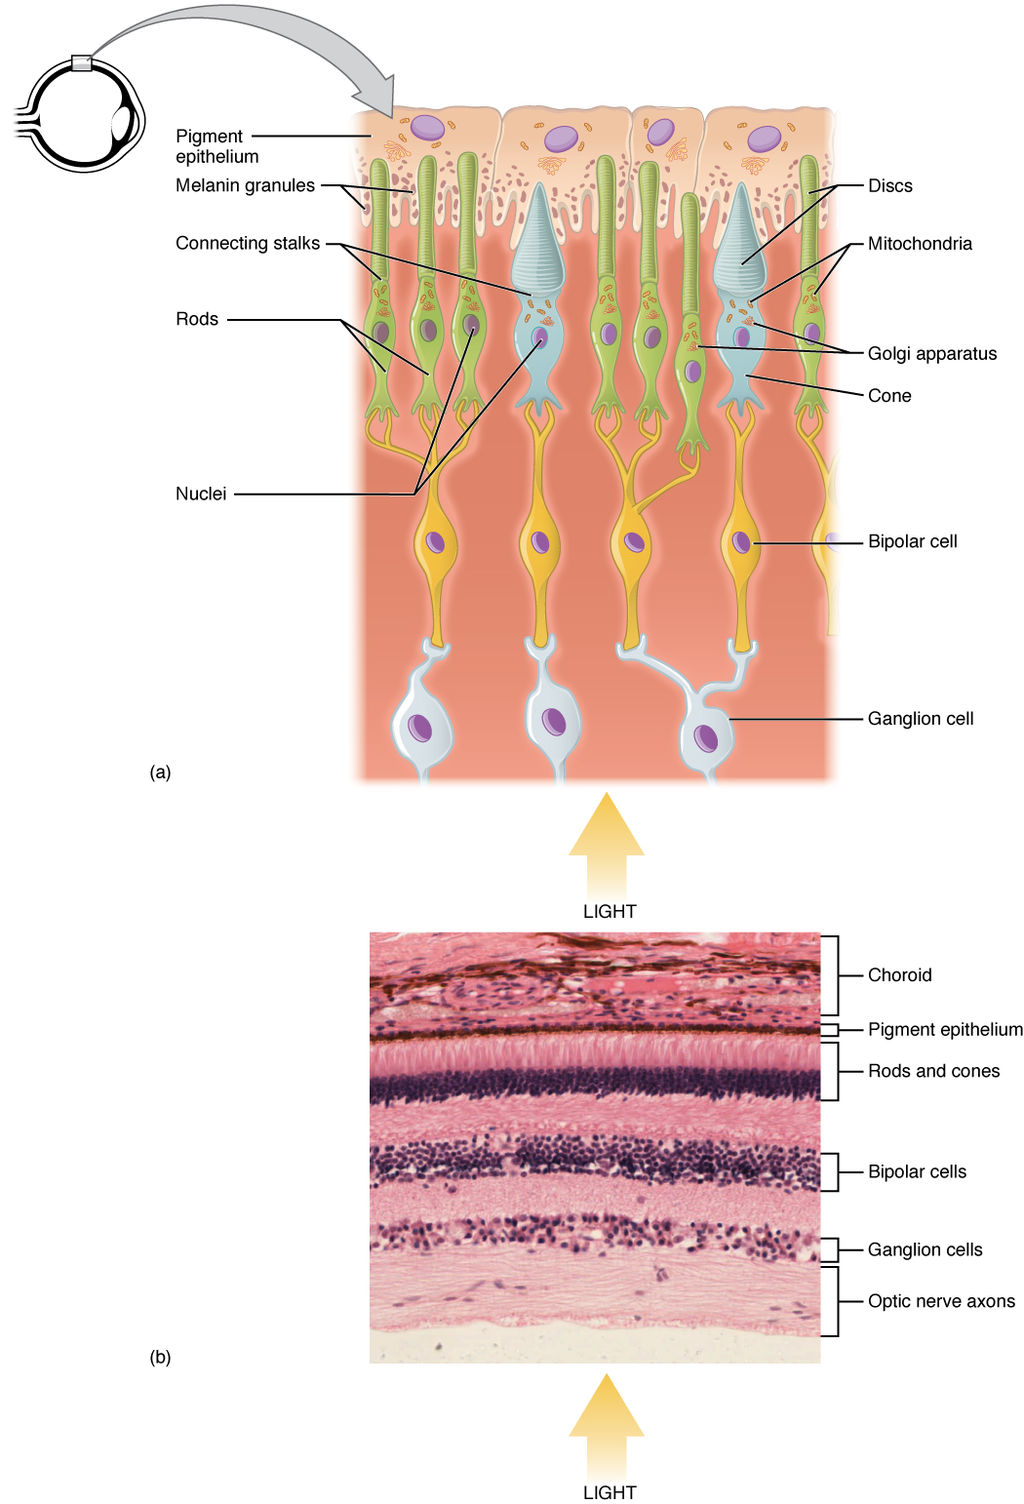
\includegraphics{figures/rods_and_cones}
  \caption{A schematic diagram of the retina with the direction of light indicated
  as being from the bottom upwards direction.}
  \label{fig:retina}
\end{figure}

There are around 0.7 to 1.5 million ganglion cells in a normal human retina.
\cite{curcio1990topography}. Retinal ganglion cells are  they are part of
the system which passes electrical signals to the brain.
\cite{meyer1995characterization} Cones and rods are photoreceptors that ensure
that light is converted into electrical signals which are transmitted to the
brain from the optic nerve, via bunches of ganglion nerves.

Whilst cones are not particularly sensitive to light, they do aid to visual
acuity by granting us colour vision.\cite{bowmaker1980visual} Conversely, cones
which have a region of pigments around $1\mu{m}$, are particularly sensitive,
even to single the pressure exerted by single photons of light at a time,
so they tend to be located around the periphery of the receptive field of
the retina.\cite{liebman1964sensitive,baylor1979responses} 
Most of the retinal cones are located around a circular trough in the
receptive field, called the fovea centralis which is located at the center
of the macular.\cite{hendrickson1994primate} It is the most sensitive part
of the eye so very few cones are located directly behind that point.
\Fref{fig:cone} shows a schematic diagram of the cone cell.

\begin{figure}[!htbp]
  \centering
    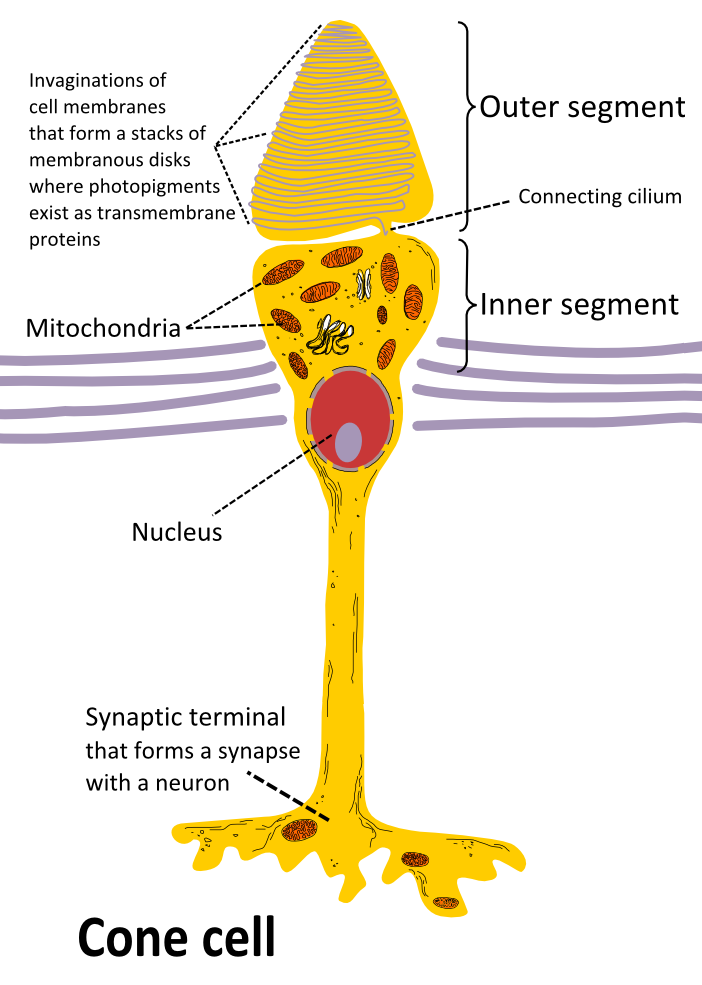
\includegraphics{cone_cell}
  \caption{A schematic diagram of the cone cell showing the outer and inner segments, nucleus
  and the synaptic terminal.\cite{wikicone}}
  \label{fig:cone}
\end{figure}

The fovea has an apparent dip, because unlike the periphery,
there are neurons situated behind it, Neurons have axons that allow electrical
signals travel to the optic nerve so they can be interpreted by the brain but
as the fovea is a particularly sensitive aid to colour vision and acuity,
axons of neurons would get in the way if they were located directly behind it.

A healthy and normal eye will pick up red, green and blue so that the brain
can interpret the full spectrum of colours, including white. \fref{fig:wavelengths}
shows normalised absorbency against wavelength for red, green and blue cones
and rods (which cannot differentiate between colours), in an average, human eye.
The range of human visual spectrum of of light lies roughly between 390nm
and 700nm.\cite{starr2010biology}.

\begin{figure}[!htbp]
  \centering
    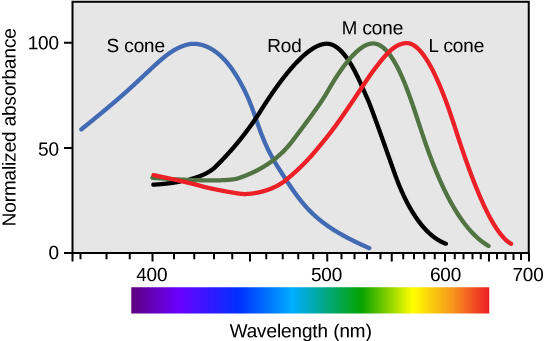
\includegraphics{wavelengths}
  \caption{Normalised absorbency vs. wavelength, for an average eye.}
  \label{fig:wavelengths}
\end{figure}

\section{Development, Dysfunction, Ageing and Disease}

During the early stages of development in babies, there is a steady
increase of a lubricating substance called glycosaminoglycan hexosamine,
in the cornea which reaches an increase plateau at around 2 years of age.
\cite{praus1975glycosaminoglycans}

Some men are born with limited functionality in cones which are
sensitive to particular frequencies of light.\cite{george1996clinical}
If all the eye cones are not working then this causes blindness
to occur but if only some types of cones have limited functionality
as photoreceptors this causes a less serious impairment, commonly
referred to as "colour blindness".

As people age, ciliary muscles weaken and this impairs the ciliary
muscles' ability to accommodate the lens and the result of this is
difficulty focusing on objects which are close by.
\cite{fisher1985ciliary}

Age related Macular degeneration of pigment cells and decreases in
Equatorial rods and ganglion cell rates are common problems affecting
central vision.\cite{gao1992aging} Macular degeneration in particular,
accounts for 95\% of blind and partial sightedness registrations in the
UK and particularly affects women.\cite{o1998age,klein2005complement}
There are two main forms of macular degeneration, non-exudative (dry)
and exudative (wet). The phenotypes in on-exudative macular degeneration
are atrophic and neovascular respectively.\cite{kuno2011dry} In
non-exudative macular degeneration, deposits build up behind the retina
resulting in its progressive thinning or scarring, with respect to time.
Exudative macular degeneration is caused by leaking of blood vessels
which causes swelling.

Preliminary studies indicate that the thickness of the choroid decreases
with age and although little is understood about how this may affect
central vision in macular degeneration, some studies have found
choroid thickness to be a predictor for open angle glaucoma which
is yet another leading cause of blindness.
\cite{margolis2009pilot,gordon2002ocular}

Glaucoma is caused by various malfunctions of aqueous humour drainage
which can lead to excessive interocular pressure bringing about damage
to the optic nerve and other vital members of the optical system.
\cite{distelhorst2003open} Open angle glaucoma happens gradually,
affecting the peripheral vision at first and progresses on to impair
central vision over time. For early diagnosis of open angle glaucoma
the relationship between interocular pressure and visual field decay
is examined by specialists to determine whether any abnormalities are
apparent so that it may be treated before permanent field damage occurs.
\cite{goldmann1972open}

Retinopathy is another common disease but one which can affect people of
all ages, by attacking the retina, A common indicator of non-proliferative
retinopathy is macular edema, symptomatic blurred vision arising from
abnormal fluid leakage and swelling in the macular from the retina's
blood vessels causing the the retina to thicken.\cite{hee1995quantitative}
Macular edema is the common cause of visual degeneration in people with
diabetes which can significantly increases a person's chance of developing
retinopathy as the diabetes progresses.\cite{klein1984wisconsin} Proliferative
diabetic retinopathy is caused by blockages in blood vessels which can can
starve the retina of oxygen. The retina responds to this by attempting to
grow blood vessels of its own, however they tend to be abnormal and hinder
fluid secretion and leak blood into the vitreous humour. Symptoms of
prolific retinopathy do not usually occur until damage has already been
done and in that case a sufferer would experience seeing "floaters",
"shadows" and loss of vision.

% Author: Matt Toman

\chapter{History of Retinal Imaging}

\label{history_retinal_imaging}
\lhead{\emph{History of Retinal Imaging}}


\section{The History of Retinal Imaging}


Direct examination of the retina is prevented by the optical properties of the eye that enable image capture and formation.  That is to say, when trying to form a retinal image from outside via an inverse imaging transform, depiction of the retina is actually prevented by the nature of the original transform which results in a focused image on its surface.

If light is shined into the eye at a certain angle, a blurred reflection of the retina can make the pupil appear to be red in colour.  This is known as the red reflex, and has been understood for hundreds of years.  Obtaining a focused retinal image is much more difficult, however, and requires specialist techniques.  The first successful attempt to acquire a retinal image was performed by Jean Mery, a French physician, in 1704.  Mery  showed that if a live cat is submerged in water, the vessels of its retina can be seen from the outside.\cite{collegeoptometrists}

Czech scientist Jan Purkinje observed the fundus of a dog and later a human eye with the use of his myopic spectacles.  Acting as a concave mirror, they reflected light into the eye from a candle situated behind the subject.  His research resulted in the realisation of the first principles of the opthalmoscope in 1823.  This was later reinvented by Charles Babbage in 1845.\cite{flick1947centenary,keeler1997150}  Babbage was also responsible for the original concept of a programmable computer, solidifying the link between retinal imaging and computing at an early stage.\cite{halacy1970charles}

The opthalmoscope was reinvented again by von Helmholtz in 1851.  As with many other important inventions, it was not based on any radical new concepts, but was a combination of several known principles.  The fundamentals of opthalmoscopy are simple.  If the subject's eye is emmetropic, or sharp and well defined, light rays which emanate from a given point on the fundus will emerge as parallel beams.  When this beam enters the pupil of an emmetropic observer the invididual rays are focused on to the obverver's retina, as shown in \fref{fig:direct_opthal}.  The result is the formation of the image of the patient's retina on the observer's retina.  This is known as direct opthalmoscopy.

%\begin{figure}[htbp]
%\centering
%  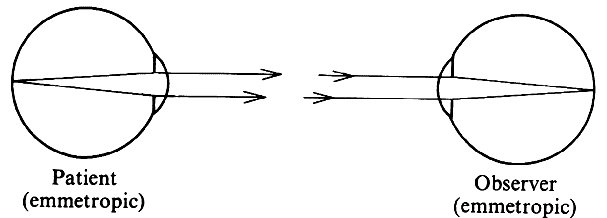
\includegraphics{figures/direct_opthalmoscopy}
%\caption{Imaging in direct ophthalmoscopy. Provided the subject and the observer are both emmetropic, rays emanating from a point in the subject's fundus will emerge as a parallel beam, focused on the observer's retina.\cite{colenbrander2013principles}}
%\label{fig:direct_opthal}
%\end{figure}


There is a significant problem with this method, however.  The patient's fundus has to be well illuminated for there to be sufficient light to visualise it.  Due to the optics of the eye, incident light can only reach the part of the fundus where the image of the light source falls.  Therefore the fundus can only be seen where the observed and illuminated areas overlap, and in the emmetropic eye this requires the light source and the observer's pupil to be optically aligned.

Fortunately there are several methods in which the illuminating and observing beams can be optically aligned, as shown in \fref{fig:illum_methods}.  The problem was solved by von Helmholtz with the use of a semireflecting mirror, made from thin pieces of glass in a parallel arrangement (A).  Epkens and Ruete used a perforated concave mirror (B), which places illuminating light rays around the observation beam.  Modern-day hand held instruments now use a small mirror or a prism, which utilises the bottom half of the subject's pupil for illumination and the top half for observation (C).


%\begin{figure}[htbp]
%\centering
%  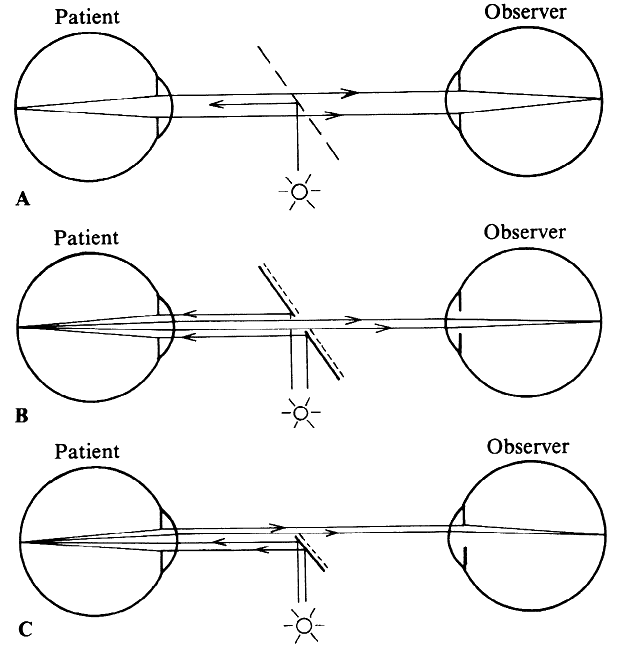
\includegraphics{figures/illumination_methods}
%\caption{Illumination methods in direct opthalmoscopy. A: Semireflecting mirror (Helmholtz). B: Perforated mirror (Epkens & Ruete). C: Prism (modern).\cite{colenbrander2013principles}}
%\label{fig:illum_methods}
%\end{figure}


The inspection and evaluation of the retina quickly became a routine excercise for ophthalmologists.  The first known image of the human retina, shown below in \fref{fig:human_retina} was published by the Dutch ophthalmologist van Trigt in 1853.  Previously, Purkinje had provided sketches of his own retinal vascalature, shown in \fref{fig:retinal_drawings}.

%\begin{figure}[htbp]
%\centering
%  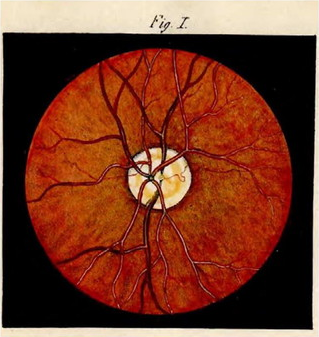
\includegraphics{figures/first_human_retina}
%\caption{First known image of the human retina, drawn by Van Trigt in 1853.\cite{van1853dissertatio}}
%\label{fig:human_retina}
%\end{figure}
%
%\begin{figure}[htbp]
%\centering
%  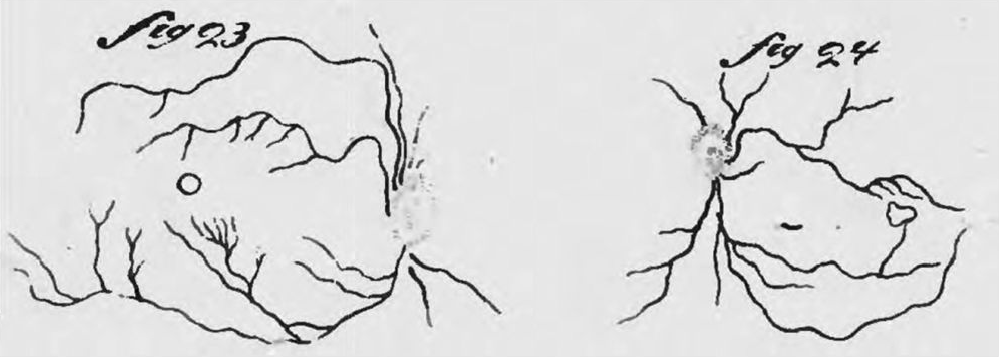
\includegraphics{figures/retinal_vasc_drawings}
%\caption{Early drawings of retinal vasculature, published by Purkinje in 1823.}
%\label{fig:retinal_drawings}
%\end{figure}

Due to the high prevalence of infectious diseases at the time, and because the ophthalmoscope necessitated the physician to be in close contact with the face of the patient, it became popular to image the eye photographically.  The first clear photographic images of the retina were obtained by German opthalmologist Gerloff in 1891.\cite{gerloffphoto}  In 1910, a Swede named Gullstrand developed the fundus camera.  He went on to receive the Nobel prize for his invention, and the concept is still utlised to image the retina in the present day.\cite{gullstrandcamera}  It has remained the primary method of retinal imaging because of how cost effective and safe it is to use.  

The next crucial development was the invention of fluorescein angiographic imaging.  A flueroescent dye is injected into the bloodstream and binds to the patient's leukocytes.\cite{novotny1961method}  A fundus camera with additional narrow band filters can then be used to capture the image.  This method has led to a better understanding of the function of retinal circulation.  However, concerns over safety have resulted in this method being slowly replaced by tomographic imaging for its primary uses, namely treatment of macular edema and macular degeneration. .

A serious limitation of fundus photography is that it only obtains a 2D representation of 3D retinal tissues, projected onto the imaging plane.  Stereo fundus photography was first described in 1964 by Allen.\cite{allen1964ocular}  This new approach relied on multi-angle retinal images combined by the human observer to derive a 3D shape.  Confocual scanning laser opthalmoscopy was later developed.  This innovation utilised a confocal aperture to obtain multiple images of the retina at different depths, yielding an estimate of its 3D shape.  Unfortunately the optics of the eye limit the depth of resolution of confocal imaging to only 100 μm, which is inadequate when compared with the typical thickness of the whole retina (300-500$\mu m$).\cite{webb1987confocal}

Tomographic imaging of the retina has become common practice following the development of femtosecond lasers, super-luminescent diodes, and, most significantly, the application of optical coherence tomography (OCT) to retinal imaging.\cite{huang1991optical}  This technique uses light to capture 3D images from within optical scattering media at micrometer-resolution, allowing for true 3D optical sectioning of the retina.\cite{van2007recent}
\section{The History of Retinal Image Processing}


Retinal image analysis methods were first examined by Matsui et al.  Their approach was grounded in mathematical morphology, utilising digitized slides of fluorescein angiograms of the retina, with a primary focus on vessel segmentation.\cite{matsui1973study}  

Many attempts to segment other anatomical structures in the eye were made in the subsequent years, all based on the use of digitized slides.  Badouin et al were the first to provide a method to detect and segment abnormal ocular structures.  In 1984 they described an image analysis method for the detection of microaneurysms, which is a characteristic symptom of diabetic retinopathy.\cite{baudoin1983automatic}  Their approach also utilised digitized angiographic images.  Microaneurysms were detected via the use of a "top-hat" transform, a step-type varient of a digital image filter.\cite{sonka1998image}  

The field of retinal image analysis changed drastically in the 1990s with the development of digital retinal imaging and filter-based image analysis techniques.  These advances in digital-based technology resulted in rapidly increasing numbers of publications.
% Author: Calum Macewen
% Tex Author: Magdalen Berns
% Formatting: Magdalen Berns

\chapter{Fundus Photography}
\label{fundus_photography}
\lhead{\emph{Fundus Photography}}


Fundus imaging is the practice of representing the 3-D retinal
tissue layers as a 2-D image through reflecting light off of
the semi-transparent tissue layers and recording the reflected
intensities. Images of the fundus (the area encompassing the
retina, optic disc, macula, fovea and posterior pole) are a key
diagnostic tool in modern ophthalmology, allowing the practitioner
to record, revisit and compare information with ease and are used
in conjunction with the clinicians own ophthalmoscope observations.
There are two principal technologies used in modern ophthalmology
to obtain fundus images: the scanning LASER ophthalmoscope and the
fundus camera. Both machines have been designed and adapted to deal
with the practical difficulties of obtaining high quality and useful
images of the retina. These two technologies deliver diverse fields
of view of the fundus and the peripheral retina, thus providing a
versatile diagnostic and prognostic tool for an ophthalmologist,
which has become necessary in the analysis and understanding of
many eye diseases.\cite{spaide2005medical}


\section{Principles of Operation}

\subsection{Fundus Camera}

The fundus camera is the original retinal imaging technology that
provided clinicians the chance to magnify the image of the retina
and record this image as a photograph via the application of indirect
ophthalmology. The modern machine comprises of an ophthalmoscopic lens
that acts as a low power microscope and a high performance commercially
available digital SLR camera to record the image formed through the
lens.\cite{shibata2003fundus} Fundus cameras are the standard machinery
for retinal imaging and devices are characterised by their angle of
view. The angle of view corresponds to the angular aperture and is a
measure of how much of the retina is imaged, with 30$^\circ$ considered
the normal angle of view, corresponding to around 12\% of the retina,
various angles of view are illustrated in \fref{fig:fov}.

\begin{figure}[htbp]
\centering
 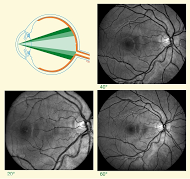
\includegraphics{figures/fieldofview}
\caption{An illustration of the standard fields of view for retinal images.}
\label{fig:fov}
\end{figure}

A key feature of the fundus camera is the manner in which it illuminates
the retina, where a peripheral zone of the retina is illuminated by a
donut of light \fref{fig:ld}.

\begin{figure}[htbp]
\centering
 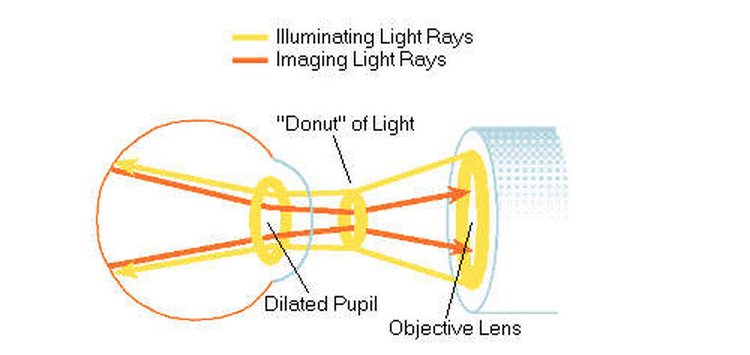
\includegraphics{figures/lightdonut}
\caption{A diagram illustrating the separation of imaging and illuminating light rays}
\label{fig:ld}
\end{figure}

This is achieved by passing the light rays of the flash through a series
of filters, lenses and mirrors. This technique allows for imaging of the
central retinal region by way of indirect illumination. Unlike an ordinary
optical system there exists the added complication of common irregularities
in patient vision such as myopia, astigmatism or hyperopia. \Fref{fig:myop}
demonstrates the optical effects of myopia.\cite{saine2002ophthalmic}

\begin{figure}[htbp]
\centering
 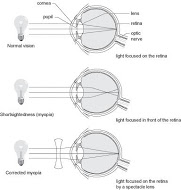
\includegraphics{figures/myopia}
\caption{An illustration of the visual effects of myopia and how it is corrected}
\label{fig:myop}
\end{figure}


The presence of these visual impairments necessitates additional lens systems
such as a dioptre compensation lens. In this report we shall look specifically
at the Topcon TRC-NW8F retinal camera, shown in \fref{fig:trc}.

\begin{figure}[htbp]
\centering
 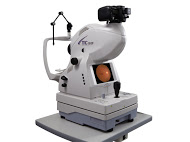
\includegraphics{figures/trc}
\caption{An image of the Topcon TRC-NW8F fundus camera}
\label{fig:trc}
\end{figure}


The TRC-NW8F is an efficient, highly specified multi-function fundus camera
that provides the clinician a variety of diagnostic tools, placing it at the
forefront of modern retinal imaging. By incorporating lens filters this device
is equipped for four imaging modes at a field of view of 45$^\circ$ with a
built-in 30$^\circ$ digital zoom feature: colour fundus, red-free, fluorescein
angiography and fundus auto-fluorescence, examples of each shown in \fref{fig:im}.

\begin{figure}[htbp]
\centering
 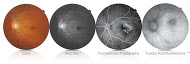
\includegraphics{figures/imagingmodes}
\caption{Comparison of the four main imaging modalities of the TRC-NW8F}
\label{fig:im}
\end{figure}


An important aspect of this device is the integrated auto focus, blink
detection and auto capture functionalities, making retinal imaging efficient
and easy to use. Capturing an image is a quick and comfortable process for
patients, where they simply rest their chin on the chinrest for a few moments
whilst the camera is adjusted to their eye position and focussed on the fundus.
The small pupil diaphragm setting on the TRC-NW8F allows for photographs to be
taken with a pupil diameter of just 3.3mm, removing the need for mydriasis in
most patients. The flash used is of low intensity to minimise patient discomfort.


\subsection{Confocal Scanning LASER Ophthalmoscope}

The confocal scanning LASER ophthalmoscope (cSLO) is a retinal-imaging device
that utilises a LASER to illuminate a small area of the retina as opposed to
the monochromatic flash of a traditional fundus camera. The mechanics of this
instrument are shown in \fref{fig:cslo}and are as follows: A LASER is generated
and passed through a lens (L1) in order to focus the beam on the retina. The
light travels through an aperture (M1), which separates the illuminating and
reflected beams. The 2-D raster (the scanning section) is created by firstly
passing the beam through a rotating polygon mirror (M2) – used to redirect
the beam horizontally to form a line – and then through a galvanometric
mirror (M3), to form the designated 2-D scanning area. The spherical mirror
(M4) focuses the raster to a point on the lens of the patient, which is then
focused on the retina by the eye, this then sweeps across the desired region
in as little as 24 milliseconds. The reflected light (dotted line) travels
back along a path identical to the illuminating beam and is returned to a
beam by the scanning mirrors (M2 \& M3). The beam is split into spectral
components by a beam splitter and focused onto a photodetector by another
lens (L2).\cite{webb1987confocal}

\begin{figure}[htbp]
\centering
 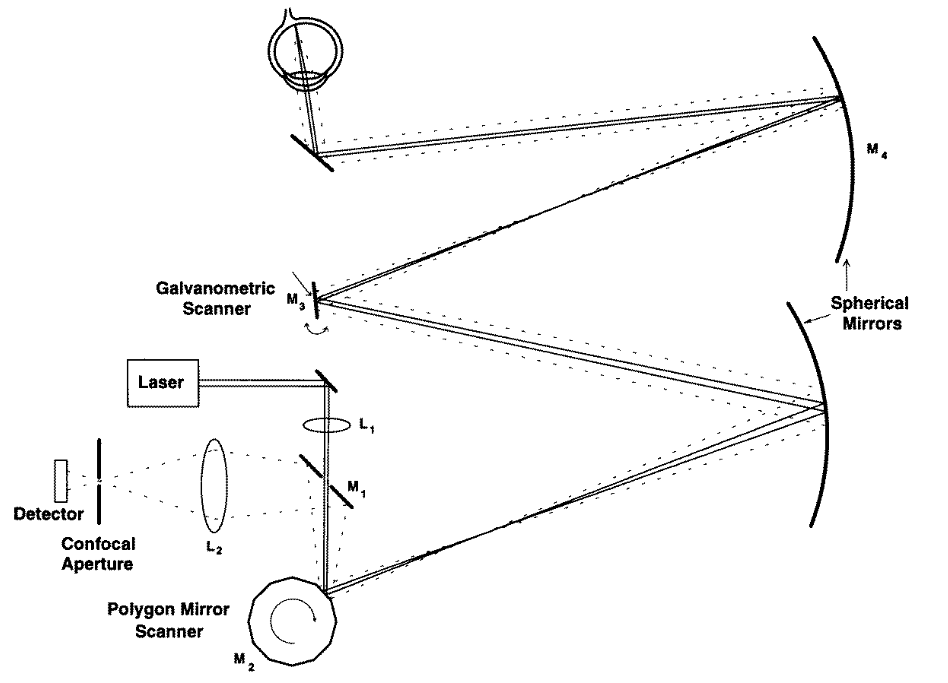
\includegraphics{figures/cslo}
\caption{Diagram showing the operating principles of a confocal laser scanning ophthalmoscope}
\label{fig:cslo}
\end{figure}


Performing multiple scans and recording the signal on the photodetector
allows for the construction of a high quality image. An integral part of
this machine is the use of a confocal pinhole (small aperture) to exclude 
eflected light that is not in the desired focal plane – hence this technology
is reliant on the principles of confocal microscopy. This technique (known as
optical sectioning) eliminates blurring and chromatic aberration as a specific
retinal tissue layer can be focussed on, with noise signal from other retinal
layers blocked by the aperture.\cite{sharp2004scanning} A further ramification
of confocal microscopy is the ability to create a 3-D image by stacking many
images of different focal lengths; hence an image illustrating the structure
of the optic nerve and retina can be assembled as is shown in \fref{fig:3dconfocal}.

\begin{figure}[htbp]
\centering
 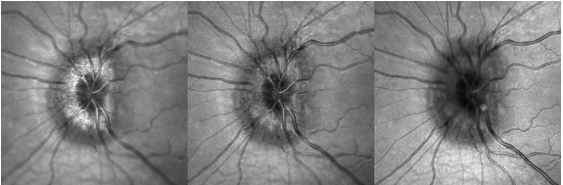
\includegraphics{figures/confocalimages}
\caption{Diagram showing how by moving the confocal plane allows for optical sectioning}
\label{fig:3dconfocal}
\end{figure}

As with the fundus camera cSLOs are characterised by their field of view,
systems operate between 15$^\circ$-200$^\circ$ without requiring the use of
an invasive lens placed on the surface of the eye. Unlike the fundus camera
however the cSLO illuminates a small circle of light with the peripheral donut
area reflecting to form the imaging beam. A comparison between the illumination
and imaging areas of a fundus camera (left image) and cSLO (right image) are
shown in  \fref{fig:illum}.


\begin{figure}[htbp]
\centering
 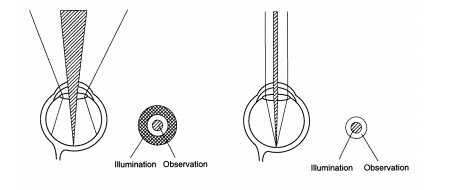
\includegraphics{figures/illumination}
\caption{An illustration of the different illumination methods used in fundus cameras (left) and cSLOs (right)}
\label{fig:illum}
    \end{figure}


This allows for much greater light collection efficiency and permits the use
of far less intense illumination beams, hence providing a more comfortable
patient experience.\cite{5_bennett_2015} This report will focus on the Optos
California ultra-wide-field cSLO, shown in \fref{fig:illum}.

\begin{figure}[htbp]
\centering
 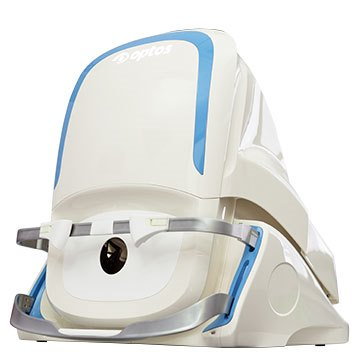
\includegraphics{figures/california}
\caption{The Optos California Ultra-Wide-Field Confocal Laser Scanning Ophthalmoscope}
\label{fig:cali}
    \end{figure}


The Optos California is a highly specified retinal-imaging device designed to
provide Ophthalmologists and Vitreoretinal Specialists with a comprehensive
diagnostic tool. This machine relies on the patented Optos ultra-wide-field
scanning technology, which through the innovative use of an ellipsoidal mirror
creates a virtual scanning point inside the eye, and can generate images with
a 200$^\circ$ field of view, as shown in \fref{fig:wideview}.  

\begin{figure}[htbp]
\centering
 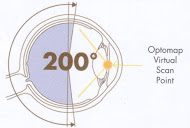
\includegraphics{figures/optoswide}
\caption{The 200 $^\circ$ Optos Optomap field}
\label{fig:wideview}
    \end{figure}

Through the assimilation of several LASER systems the California has numerous
imaging modalities, namely: fluorescein angiography, fundus auto-fluorescence,
ultra-wide-field colour fundus, central pole fundus, indocyanine green
angiography and red-free.\cite{7_burnett_hodd_2012} Taking images with the
California is simple and quick; the patient places their chin on the chinrest
and the clinician adjusts their position with the assistance of visual alignment
software, the image is then compiled from multiple scans and displayed on the
clinicians screen in under a second. Images are typically obtained without the
need for mydriasis due to the optical design; hence this machine is beneficial
for patients who dilate poorly, such as diabetics. A comparison of zero dilation
\cite{11_de brouwere_2013} images taken with a cSLO (left) and a fundus camera
(right) is shown in \fref{fig:zero}.  

\begin{figure}[htbp]
\centering
 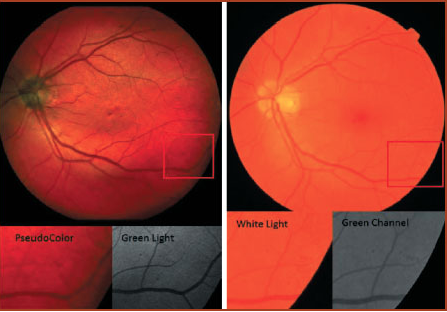
\includegraphics{figures/zerodilation}
\caption{Zero dilation images with a cSLO(left) and standard fundus camera (right)\cite{11_de brouwere_2013}}
\label{fig:zero}
    \end{figure}



\section{Practical Difficulties}

Imaging the retina presents a series of unique technical problems compared
with more commonplace photography. The primary difficulties are the turbidity
of the ocular tissue (such as cataracts in the lens), the constrained aperture
size as a result of the relatively small pupillary opening, the inability of
illumination and imaging light to intersect and the fundamental challenge of
representing a curved 3-D structure as a 2-D image.

As outlined previously, cataracts are a symptom of age related eye changes,
where the lens becomes opaque and thus reduces the visual field of the patient,
shown in \fref{fig:cat}. If the cataract is located over the pupil then this
biological phenomena can altogether prevent the capturing of a retinal image,
akin to covering the object of a photograph with a veil, hence blocking the
illuminating light from penetrating the outer surface of the eye and onto the
retina. This is a problem for both instruments and is solved by the removal
of the cataracts via surgical procedure. The California ultra-wide-field
scanning laser ophthalmoscope does provide more scope for imaging with
cataracts present, as the scanning LASER is able to penetrate the hazy
tissue.

\begin{figure}[htbp]
\centering
 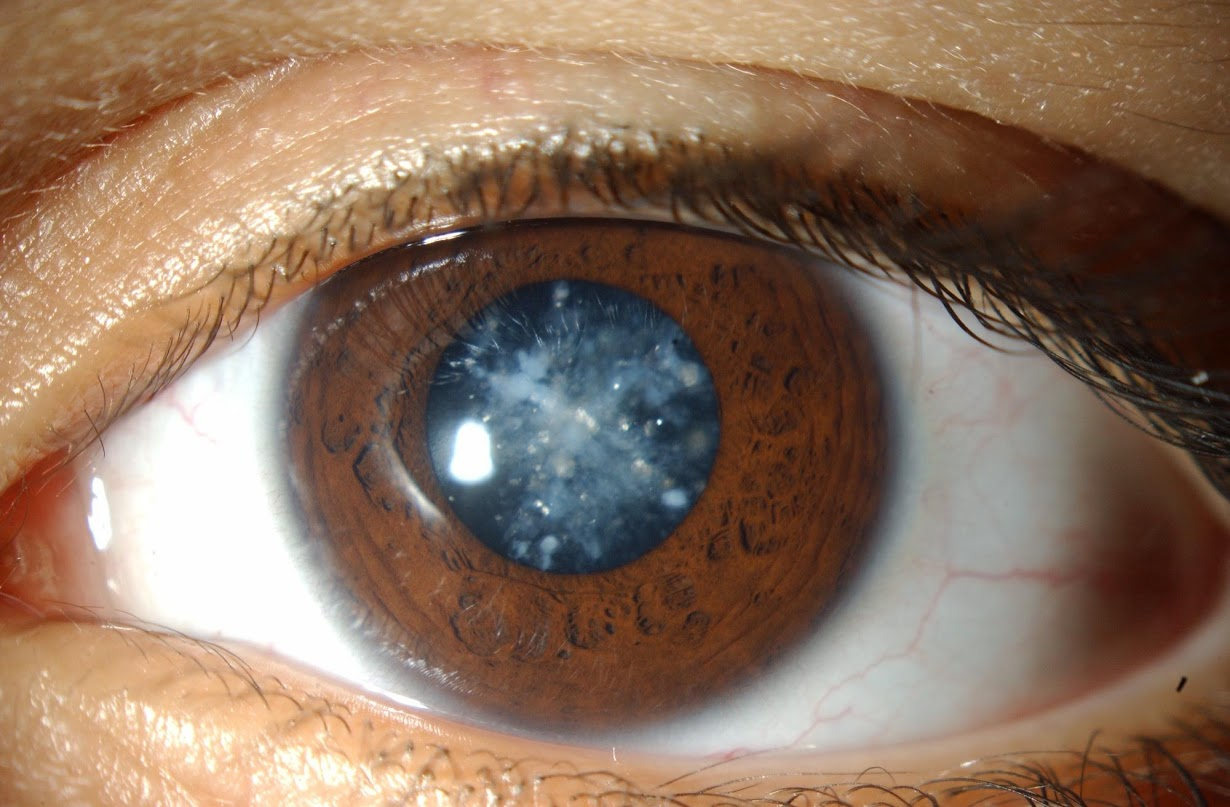
\includegraphics{figures/cataract}
\caption{Image showing the clouding of the lens as a result of a cataract}
\label{fig:cat}
    \end{figure}

Aperture size is the physical limitation of the optical system that
constrains the amount of light available for capture through a lens,
where available light is proportional to aperture area, which is in
turn related to the optical system is shown in \eref{eq:optical_system}

\begin{equation}
A = \pi({\frac{f}{2N}})^2
\label{eq:optical_system}
\end{equation}

where A is the area of the aperture, N is the f-number (ratio of lens'
focal length to diameter of entrance pupil) and f is the focal length
of the lens. This relationship is applicable to the case of the fundus
camera, where expanding the pupillary opening reduces this constraint.
To maximise the pupillary opening the patient is photographed in a dark
room where pupil diameter can be between 3-8mm, dependent on age. If this
effect is insufficient then an increased pupil diameter is chemically
induced through the use of mydriatic eye drops, which relax the constrictive
nerves, shown in \fref{fig:myd}.

\begin{figure}[htbp]
\centering
 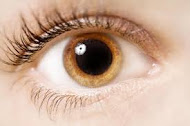
\includegraphics{figures/mydriasis}
\caption{Image showing the effect of mydriatic medicine on the pupillary opening}
\label{fig:myd}
    \end{figure}
The cSLO does not image in this manner, as was outlined earlier, and is
therefore not described by this relationship, hence removing the need for
mydriasis and greatly improving patient comfort and procedure time.

As the pupil is the only opening through which the retina can be
observed, light is required to enter and leave through the same
optical path, consequently care has to be taken to avoid ray overlap
otherwise the image will have reduced or zero contrast. Gullstrand
first introduced this idea in 1910, where he stated that to avoid
scattering between the two beams they must be entirely unconnected
across the optical path. He further specified that bright corneal
reflections are the result of scattering on the corneal plane,
whereas scattering from lens surfaces and opacities occur as the
light rays penetrate the lens. This challenge is overcome in
both machines but with different methodologies, as was described
and illustrated in the previous section.

Accurate 2-D representation of the 3-D retinal tissue structure
poses a significant challenge in both devices. Images taken by the
fundus camera are centred on the posterior pole, hence they must
demonstrate to some degree the foveal depression in the centre of
the macula, along with the depth of the optic nerve head. In a standard
fundus image such as \fref{fig:standard}the dark circular area in the
centre of the image distinguishes the foveal dip, but illustrates
nothing of the actual depth of the depression. Nor does it show any
depth of the optic nerve as its reflective properties differ to that
of the surrounding retinal tissue.

\begin{figure}[htbp]
\centering
 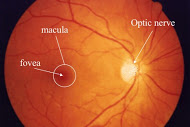
\includegraphics{figures/normalfundus}
\caption{Image showing a  standard fundus image, highlighting areas of significant depth}
\label{fig:standard}
    \end{figure}

This issue resulted in the development of stereo fundoscopy, where
two similar images are taken from different positions, corresponding
to the left and right eye of the photographer, shown in \fref{fig:stereo}.
When processed these images are viewed side by side and the brain
reconstructs a 3-D image by recognising the depth differences.\cite{tyler1997stereo}
This method cannot however provide the same degree of depth perception
as in indirect ophthalmoscopy.

\begin{figure}[htbp]
\centering
 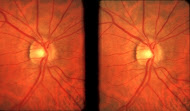
\includegraphics{figures/stereo}
\caption{Image of a stereo fundus photograph}
\label{fig:stereo}
    \end{figure}

In the ultra-wide-field cSLO there is the added difficulty of flattening
the curved surface without incurring a drastic reduction in proportional
accuracy, something known amongst cartographers as the ‘Greenland effect’.
This challenge is dealt with in the Optos California by corrective imaging
software. As the Optos California is able to perform optical sectioning it
is possible to generate a 3-D image of the retina and optic nerve by moving
the desired focal plane through the back of the eye, shown in\fref{fig:3d}.
The accuracy of these images is significantly limited by the depth resolution
of the machine, which is around 100 micrometres, corresponding to  a large
fraction of the entire retinal thickness (300-500 micrometres).

\begin{figure}[htbp]
\centering
 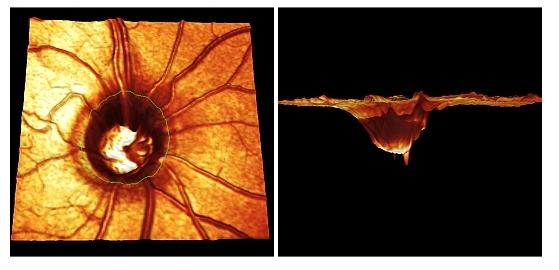
\includegraphics{figures/3dcslo}
\caption{Illustration of a 3-D image formed by confocal optical sectioning}
\label{fig:3d}
    \end{figure}

It was these inaccuracies and shortcomings in 3-D retinal imaging that
led to the development of independent tomographic scanning devices such as the OCT.


Imaging Modalities and Their Diagnostic Significance

The Optos California and Topcon TRC-NW8F are machines that house multiple
imaging modalities, with each function serving a different clinical need.
There are four main modalities: colour fundus, red-free, fluorescein angiography
and fundus auto-fluorescence. The Optos California develops the scope of these
modalities by capturing an ultra-wide-field image; hence this feature will be
examined as a fifth modality of interest.


\section{Colour Fundus}

Colour fundus images focus on the retina and produce an image of the vascular
network and optic nerve head. This is the normal operating image modality for
the TRC-NW8F, where a full colour image of the retina is obtained as a result
of the white light used to illuminate the subject area, shown in \fref{fig:cf}.
The Optos California produces colour fundus images by illuminating the retina
with a green and a red laser and combining these reflections, hence it is not
a true full spectrum colour image, as is clear from \fref{fig:cfoptos}.

\begin{figure}[htbp]
\centering
 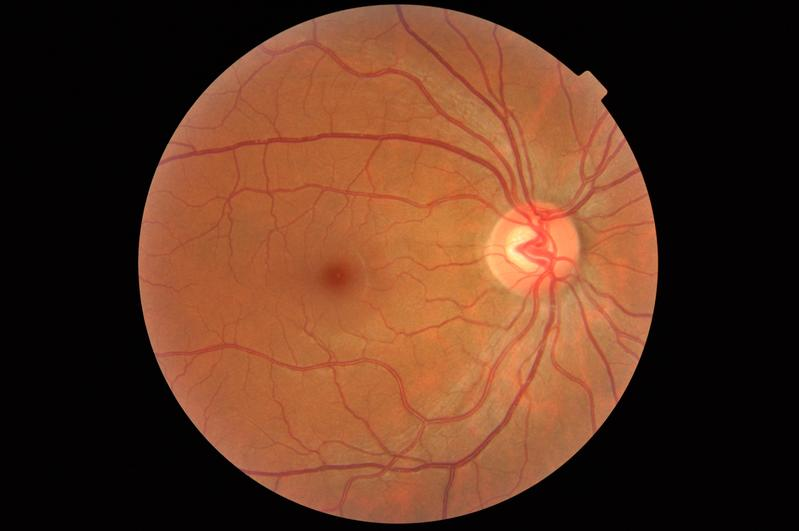
\includegraphics{figures/colourtrc}
\caption{A colour fundus image of a healthy eye, taken with the TRC-NW8f}
\label{fig:cf}
    \end{figure}

\begin{figure}[htbp]
\centering
 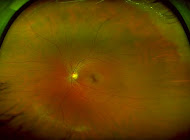
\includegraphics{figures/optoscolour}
\caption{A colour fundus image of a healthy eye, taken with the Optos California}
\label{fig:cfoptos}
    \end{figure}


From a clinical perspective colour fundus imaging is the first port of call
for diagnosis of many ocular diseases, namely diabetic retinopathy, age
related macular degeneration (AMD), retinal detachments and optic nerve abnormalities.\cite{3_medicine.uiowa.edu_2015} The clinician’s observations of these
images direct the line of investigation, with the majority of common
ocular pathology observable in this mode. Due to the increasing prevalence
of diabetes in modern society - and thus diabetic retinopathy - the Scottish
government introduced a national diabetic screening programme to detect early
signs of the disease and reduce the likelihood of blindness and proliferation.
Diabetic retinopathy is a progressive eye disease that causes bleeding and
fatty fluid leaks in the retina illustrated in \fref{fig:dr}, which ultimately
develops into diabetic macular oedema if left untreated. Colour fundus images
are therefore at the frontline of diabetic retinopathy detection and are an
invaluable tool in saving the vision of many patients.

\begin{figure}[htbp]
\centering
 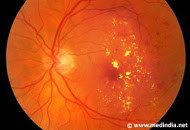
\includegraphics{figures/diabeticretinopathy}
\caption{A colour fundus image of diabetic retinopathy. The red patches indicate haemorrhages and the yellow areas show fatty fluid leakage.}
\label{fig:dr}
    \end{figure}

Colour fundus images are also essential in the diagnosis of glaucoma and
papilledema, conditions that visually affect the appearance of the optic
nerve disc head.  In the case of papilledema heightened intracranial pressure
results in swelling of the optic disc, which is immediately apparent on a
fundus image, demonstrated in \fref{fig:pap}. Early diagnosis of this condition
is vital not just for preserving the vision of the patient but also in identifying
the presence of a systemic disease – papilledema is often a side effect of brain
tumours and respiratory issues. For glaucoma, colour fundus imaging is used in
the monitoring of so called ‘optic nerve cupping’. This is a result of increased
intraocular pressure, which causes the central section of the optic nerve – known
as the cup – to become enlarged. Ophthalmologists rely on fundus images to document
the cup-to-disc ratio, which is key in assessing the efficacy of current treatment.
\Fref{fig:cup} shows the enlargement of the cup over time.

\begin{figure}[htbp]
\centering
 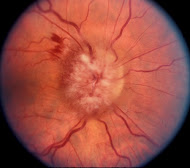
\includegraphics{figures/papilledema}
\caption{A colour fundus image of papilledema. The optic nerve head is noticeable larger and swollen.}
\label{fig:pap}
    \end{figure}

\begin{figure}[htbp]
\centering
 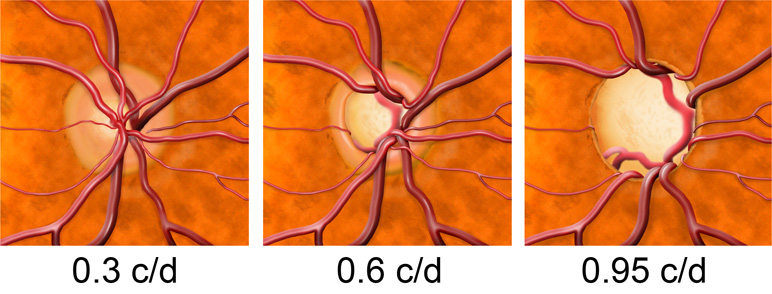
\includegraphics{figures/opticnervecupping}
\caption{An illustration of increasing cup-to-disc ratio in the optic nerve head.}
\label{fig:cup}
    \end{figure}

	

\section{Red-Free}

This modality (also known as monochromatic fundus imaging) uses a monochromatic
LASER or filtered light source to illuminate the retina. As the various retinal
tissue layers have different absorption and reflection properties one illumination
frequency can be used to highlight a specific region of interest. This technique
boosts the contrast between retinal features and provides the clinician with a
useful tool for examining individual features of the retina. Red-free specifically
relates to the use of a green filter or in the case of the Optos a green LASER,
which illuminates the retina at a wavelength of 540nm.\cite{4_bennett_2015}
A great number of visual defects and eye diseases are borne from issues in
the vascular network, where clotting and lesions result in partial visual
field loss or blindness. The clinician is thus highly concerned with obtaining
images that illustrate the presence of blood in the retina, whilst minimising
noise reflections that reduce the overall image contrast. Green light is the
ideal wavelength choice for this task as it is strongly absorbed by blood,
whilst moderately reflected by the retinal pigment epithelium. This creates
high contrast images that clearly illustrate the flow of blood in the retina
as shown in \fref{fig:red} and \fref{fig:reddr}; hence this is an essential
imaging mode for practitioners, allowing simple and quick documentation of
the vascular network. Red-free is also suitable for imaging when there exists
a degree of ocular turbidity, as there is less scatter present compared with
shorter wavelengths.

\begin{figure}[htbp]
\centering
 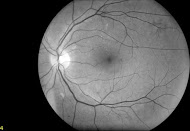
\includegraphics{figures/redfree}
\caption{A red-free image of a healthy retina.}
\label{fig:red}
    \end{figure}

\begin{figure}[htbp]
\centering
 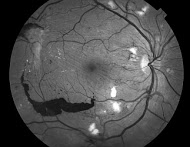
\includegraphics{figures/redfreediabetic}
\caption{A red-free image of a patient suffering from diabetic retinopathy. The large haemorrhages and fatty fluid leaks are clearly identified in this mode.}
\label{fig:reddr}
    \end{figure}



\section{Fluorescein Angiography}

Fluorescein is a soluble synthetic compound used as a dye tracer in
several medical applications, principally because of its relative inertness.
In fluorescein angiography an amount of sodium fluorescein is injected into
the patient and the resulting progression of the dye through the vascular
network is imaged or recorded over a set time frame. The dye normally takes
around 12 seconds to appear in the arteries of the retina then after 5 seconds
moves through into the capillary vessels and veins. \Fref{fig:fluor} shows
complete vascular and arterial dye diffusion.

\begin{figure}[htbp]
\centering
 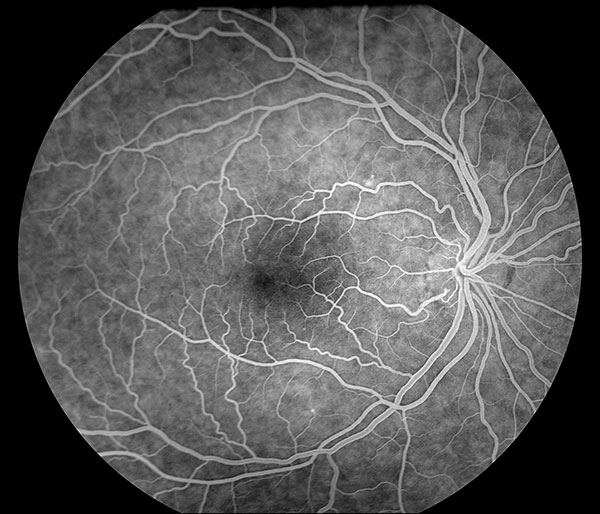
\includegraphics{figures/fluoresceinangio}
\caption{A fluorescein angiogram of a healthy eye.}
\label{fig:fluor}
    \end{figure}

Fluorescein is strongly absorbing of light with a wavelength of 494nm and
through the process of fluorescence emits light with a frequency of 520nm.
Through the use of a blue illumination light and an excitation filter high
contrast images of blood flow in the retina and choroid can be captured.
The excitation filter prevents light from being imaged with a wavelength
below 520nm thus avoids capturing any reflections from the illuminated tissue.
\cite{demofluorescein} The clinical motivation for red-free imaging is applicable
to fluorescein angiography as they both seek to highlight the presence of blood
in the retina, with this modality capable of providing greater detail of small
capillary lesions, \fref{fig:fluordr} shows microaneurysms symptomatic of diabetic
retinopathy. Along with illustrating vascular pathologies this modality can provide
a measurement of the patients blood flow, often used in the diagnosis of general
cardiac problems. 

\begin{figure}[htbp]
\centering
 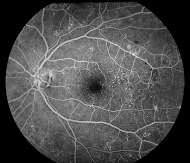
\includegraphics{figures/fadiabetic}
\caption{A fluorescein angiogram illustrating small capillary lesions in a patient suffering from diabetic retinopathy.}
\label{fig:fluordr}
    \end{figure}

\section{Fundus Autofluorescence (FAF)}

As a result of fluorescein angiography procedures ophthalmologists noticed
that areas of the fundus were fluorescent without the use of any dye tracer.
This weak autofluorescence was subsequently identified as a valuable diagnostic
criterion and plays an important role in the monitoring of disease advancement.
The method for imaging in this mode is similar to that of fluorescein angiography,
where in the case of the fundus camera an illumination beam is absorbed by
fluorescent tissue, which then emits photons of higher wavelength, allowing
for the effective filtration of insignificant reflections. cSLOs work along
the same principal but provide the additional benefit of selecting the focal
plane of interest.\cite{schmitz2008fundus} This feature is particularly relevant
for fundus autofluorescence as it removes any specious fluorescence originating
from other ocular tissue, principally the lens as it contains a small element of
fluorescent material. \cite{von1995distribution} The primary aim of this imaging
modality is to observe the accumulation of lipofuscin in the retinal pigment
epithelium, which can signal a variety of issues. Lipofuscin is fluorescent over
a broad range of wavelengths therefore the illumination beam is not as restricted
as in the case of fluorescein angiography. Recently developments have been made
with the use of near infrared illumination beams to excite melanin, providing
yet more information about the distribution of organic materials in the retina.

To understand the clinical significance of FAF imaging we must first understand
the process of lipofuscin build up.\cite{kennedy1995lipofuscin} Age-related
degeneration or disease can cause photoreceptors in the retina to become
damaged and in response will expel an outer layer of tissue, which is
subsequently absorbed by the retinal pigment epithelium (RPE).\cite{spaide2003fundus}
The accretion of these molecules (or lack of) creates lipofuscin deposits
in the RPE, which can be used to characterise the retina either through
observing hyperfluorescence or hypofluorescence.\Fref{fig:faf} shows a
fundus auto-fluorescence image of a normal retina, where the natural
build up of lipofuscin in the RPE is clearly observed.

\begin{figure}[htbp]
\centering
 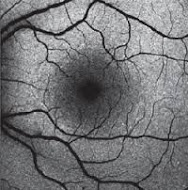
\includegraphics{figures/faf}
\caption{A confocal laser scanning ophthalmoscope FAF image of a normal retina. The lack of fluorescence from the macula is a result of absorbing pigmentation in this area. Retinal vessels block the reflection from the RPE beneath them so appear dark.}
\label{fig:faf}
    \end{figure}

Hyperfluorescence can be attributed to an increase in the rate
of shedding of photoreceptor outer segments or a breakdown in
the ability of the RPE to process these cells. Hypofluorescence
is indicative of cell death in the RPE, known as geographic atrophy.
age related macular degeneration (AMD) results in the thinning and
degradation of the RPE and so this geographic atrophy is directly
observable with FAF imaging, illustrated in\fref{fig:fafamd}.

\begin{figure}[htbp]
\centering
 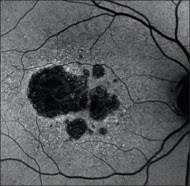
\includegraphics{figures/fafamd}
\caption{A FAF image of a patient suffering from dry AMD. Age-related macular degeneration causes both hypo and hyperfluorescence, as a consequence of geographic atrophy and the resulting increased work of surrounding retinal tissue.\cite{2_audo_2015}}
\label{fig:fafamd}
    \end{figure}

The ability to demarcate between geographic atrophy and healthy retinal tissue makes FAF imaging a valuable prognostic tool, which is commonly used in the evaluation of treatment and the monitoring of dry AMD progression.\cite{1_murphy_2015}

\section{Ultra-Wide-Field Imaging}

Ultra-wide-field images greatly expand on the standard field of view and are
capable of capturing images of the peripheral retina. Until recently
non-contact imaging technology was unable to capture images with more
than a 50$^\circ$ field. \Fref{fig:uwfc} illustrates the disparity of
field of view amongst retinal imaging devices. The clinician was thus
unable to visually record any pathology directly observed in the peripheral
retina through their ophthalmoscope. Advancements in technology have opened
up this area for documentation, with peripheral retinal imaging now forming
an important part of disease detection and monitoring.\cite{8_sides_media_2015}

\begin{figure}[htbp]
\centering
 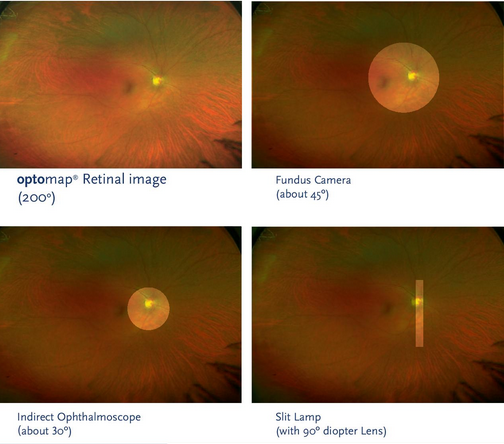
\includegraphics{figures/uwfcomparison}
\caption{A comparison of the imaging areas for various retinal imaging devices.}
\label{fig:uwfc}
    \end{figure}

Both the Optos California and the Topcon TRC-NW8F are capable of producing
wide-field images through differing methods. The Topcon TRC-NW8F employs
the traditional non-contact method of wide-field imaging: it sets out 9
fixation targets on the retina, takes individual photographs of each area
then pieces these photographs together using the auto-mosaic software to
give a 75$^\circ$ field. The Optos California operates in an entirely
different way, employing its patented ultra-wide-field scanning technology
to capture one complete 200$^\circ$ field. \Fref{fig:uwfvs} displays the
difference in the wide-field images these devices can capture.

\begin{figure}[htbp]
\centering
 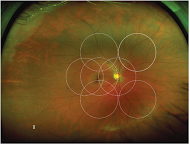
\includegraphics{figures/uwfvs}
\caption{The 200 degree Optos visual field compared with the 75 degree field of the fundus camera. Illustrative of the Optos' superiority in imaging the peripheral retina.}
\label{fig:uwfvs}
    \end{figure}

By combining this modality with other modalities, primarily fluorescein
angiography, the Optos presents a clear clinical advantage over other
devices. As discussed previously the progression of the dye through the
retina’s circulation occurs in a short period of time; hence the piecemeal
image formation of the fundus camera is ineffectual at capturing an accurate
depiction of peripheral blood flow, as image capture is limited by the time
to move the camera. The Optos California is capable of capturing the entire
field in one image and recording a video of the dye progression through the
retina, which is of significant medical use.

From a clinical perspective the ability to capture ultra-wide-field images
is incredibly advantageous in the diagnosis of many retinal pathologies
\cite{6_witmer_kozbial_daniel_kiss_2012} and presents ophthalmologists
with a tool to detect signs that would have otherwise gone unnoticed, such
as the pathology in the far left of \fref{fig:uwfdr}.

\begin{figure}[htbp]
\centering
 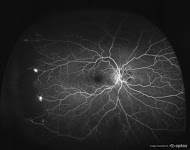
\includegraphics{figures/uwfdr}
\caption{An ultra-wide-field fluorescein angiogram of a patient suffering from diabetic retinopathy. The expanded field of view allowed for the detection of the peripheral pathology.}
\label{fig:uwfdr}
    \end{figure}

Recent studies have sought to evaluate the implications of ultra-wide-field
imaging for the detection and prognosis of diabetic retinopathy. One study
found that detection was increased by 17\% compared with standard fundus images,
with the classification of disease severity augmented in 9\% of cases due to the
detection of peripheral lesions. \cite{silva2014potential}

\chapter{Optical Coherence Tomography}

\label{optical_coherence_tomography}
\lhead{\emph{Optical Coherence Tomography}}

Optical Coherence Tomography (OCT) is an important advancement in retinal imaging
technology.  Research leading to OCT technology was made possible during the
1980’s with advancements in the fibre-optics and photonics industries, allowing it to be
developed in 1991 by David Huang and colleagues.\cite{mbib_1,mbib_2,mbib_3} 
Since 1991, many improvements have been made to enable high quality and detailed 
scans of retinal tissues.  The retina, as mentioned previously, is made up of twelve
internal layers with a total thickness between 300-500 $\mu m$.\cite{mbib_4}
These layers are important indicators for monitoring and diagnosing retinal diseases,
which is why opticians use technologies such as OCT to image retinal tissues.

OCT is a non-invasive imaging technique “analogous to ultrasound,” relying on low 
coherence (also referred to as “white light”) interferometry to generate cross-sectional
imagery (or tomography) of retinal tissues within the eye to a “micrometre axial
resolution” of 1-15 micrometres.\cite{mbib_5, mbib_6,mbib_2} Unlike a normal camera,
which only has transverse dimensional resolution, OCT imaging uses low coherence
interferometry to estimate the origin of specific backscatter [from the source of light]
within the retina.\cite{mbib_4}  In other words, OCT images depth as opposed to simply
taking an image of the surface.  Depth resolution can be carried out using three main
methods: Time-domain OCT (TD-OCT), Fourier-domain OCT (FD-OCT) and
Spectral-domain OCT (SD-OCT).  The latter two are normally combined as they are very
similar methods, therefore for simplicity and consistency they will jointly be referred to as
Spectral-domain OCT (SD-OCT).

In the following sections the physics behind OCT technology will be explained further
and the different methods will be described as well as a discussion on image analysis for
different medical diagnostic purposes.

\section{Low Coherence Interferometry}
Because the velocity of light is much larger than that of the
distance between the retinal layers, it is not possible to
directly measure the flight-time of the light returning from the retinal
tissues. \cite{mbib_5} Meaning, the incoming and outgoing light
cannot be differentiated without
the use of low coherence interferometry. Low coherence interferometry
is just as it sounds.  A low coherence light beam, which can be thought
of as a “train of highly autocorrelated overlapping ‘bursts’ of light,”
is directed at a sample surface using an optical probe, which is connected
to the interferometer.\cite{mbib_4}  When the light “burst” hits the
transparent sample, light will be reflected off of the layers within
the sample and its unique autocorrelogram will be detected by its
autocorrelation function to get an idea of the structure of the sample.
\cite{mbib_4,mbib_3,mbib_6} It should be noted that these “bursts” are a
way of explaining what is happening, and are not to be thought of as a
pulsed light source.

In \fref{fig:m_1}, a schematic of the low coherence interferometer used in the classic and current OCT imaging can be found.

\begin{figure}[htbp]
\centering
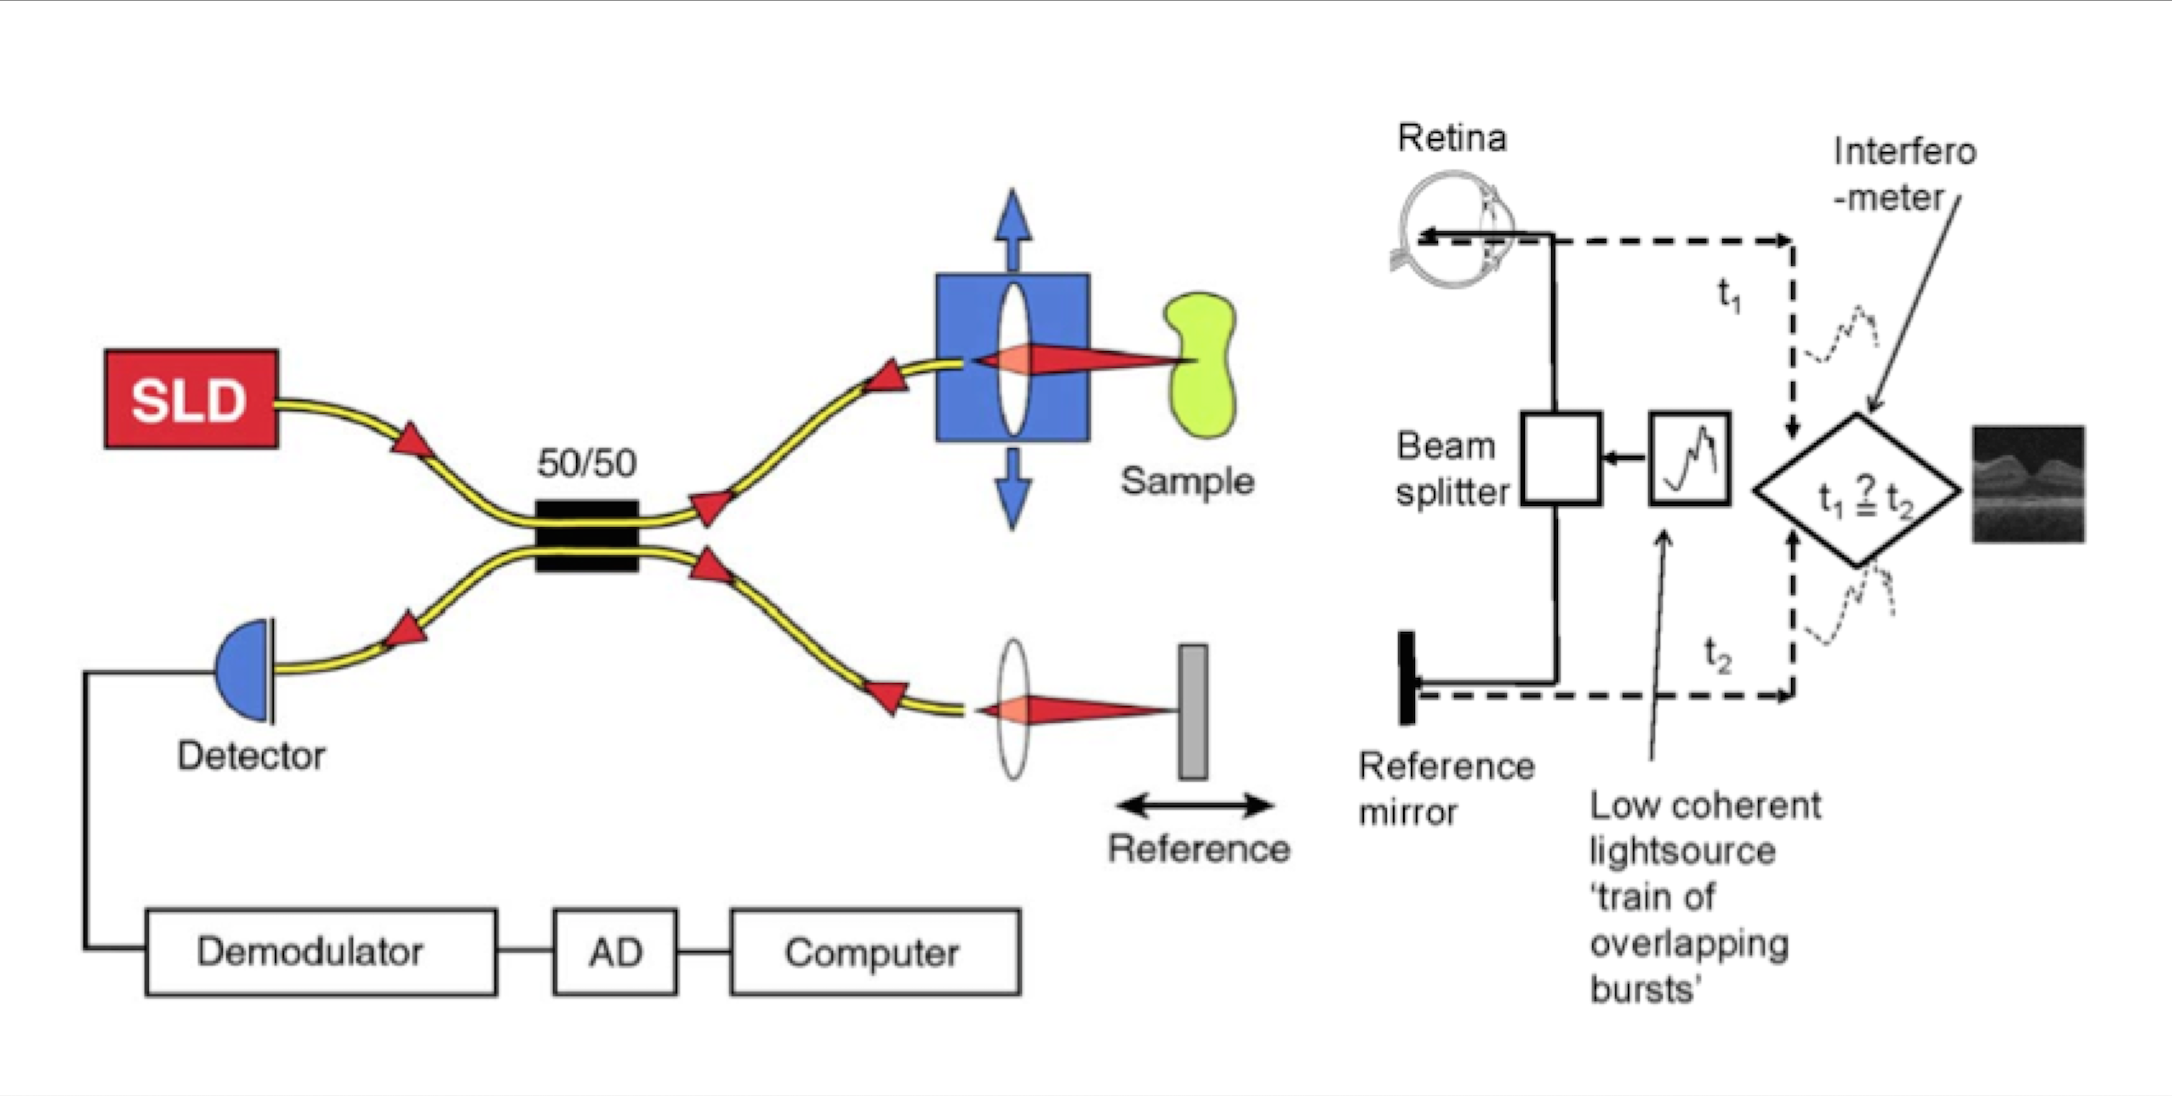
\includegraphics{figures/morgan_1}
\caption{(Left) Classical optical coherence tomography system. 
(Right) A schematic of an optical coherence tomography set-up with particular emphasis on the splitting of light and their interface after being reflected from the retinal tissues as well as from the reference mirror.  An assumption that the time delays of both paths are equal. \cite{mbib_6,mbib_4} }
\label{fig:m_1}
\end{figure}


Super-luminescent LEDs (SLED), also known as super-luminescent diodes (SLD),
which produce wavelengths which reside in the near infrared region, are
traditionally used in OCT interferometry because they are “economical,
compact, long-lasting, and emit high quality beams that couple efficiently
with an optical fibre.” \cite{mbib_6} Also, the amount of light coherence
is inversely proportional to the depth resolution, thus wavelengths longer
than visible light, typically 800–1400nm wavelengths in the near infrared,
are necessary as they penetrate deeper into the retinal tissue layers.\cite{mbib_4,mbib_7}
The resolution of the generated images is limited by the progress of SLD
technology, for example, early systems used SLDs emitting wavelengths around
820 nm, limiting the axial resolution to 11 mm in retinal tissues and 15 mm
in air. \cite{mbib_6}  Today, the CirrusTM HD-OCT device uses SLDs with wavelengths
of approximately 840 nm, and achieve a resolution of 5 mm in retinal tissue.\cite{mbib_7}

Inside the interferometer, the light from the SLD is split using a beam splitter.
Other splitting methods such as a 50/50 fibre coupler can be used, but the beam
splitter is the most commonly used method to date.  When the light from the SLD
is split, half of the light is directed to a reference reflective mirror at a
specific distance, while the other is directed into the retinal tissues (sample)
using an optical fibre.  The returning beams from the reference and sample arms
are recombined and produce interference when the distance in the two paths is
equivalent within the coherence length of the light source. \cite{mbib_5,mbib_6}

The interference of two incoming waves can be thought of as the addition of their
respective amplitudes, which is also commonly known in physics as superposition.
When the two waves are in phase, constructive interference occurs and their combined
waveform can be called coherent.  This constructive interference leads to the two
returning waves in the interferometer adding to produce a large interferometric
modulation.  On the other hand, the two returning beams could be largely misaligned
and interfere destructively, with an extreme of them adding up to a flat line.
As the galvanic reference mirror with freedoms in the x and y directions is moved,
the phase of the reference wave changes, and produces a sinusoidal interference
signal, see \fref{fig:m_2}. The summed interference signal forms a wave pulse 
that is converted
from light into an electrical current using a photodetector (light sensor).\cite{mbib_6}
The information is then processed electronically to extract the pulse envelope, which
is then transferred to a computer where it is stored on the memory.\cite{mbib_6}

\begin{figure}[htbp]
\centering
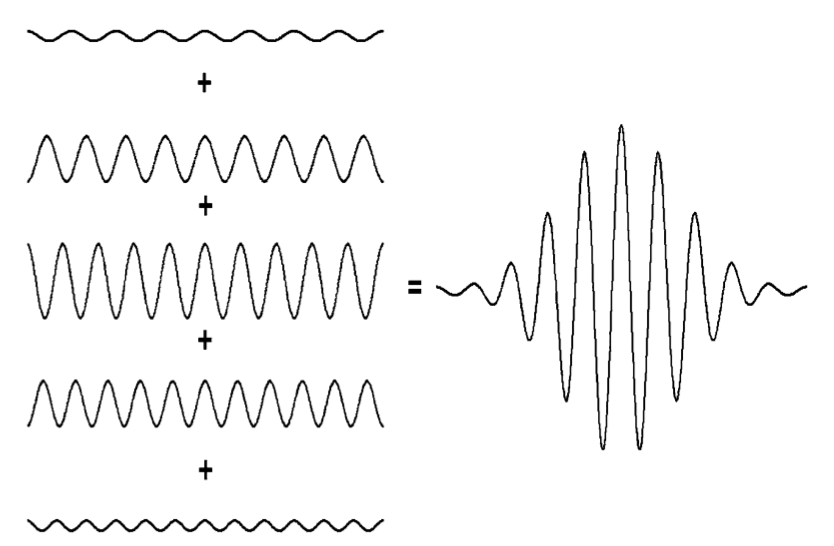
\includegraphics{figures/morgan_2}
\caption{The combined interference signal of a range of wavelengths (left) is 
shown on the right.  The width of this pulse determines the axial resolution of 
the OCT device. \cite{mbib_6} }
\label{fig:m_2}
\end{figure}

The pulse envelope’s width reveals the coherence length by providing
the coherence time (time of flight).  The coherence length can be found
by multiplying the time of flight by the speed of light, and is an
important quantity as it determines the axial resolution of the OCT
device. \cite{mbib_6}  By scanning the retina and recording this
information, a plot of the amplitude against the delay can be generated to
demonstrate tissue reflectivity at successively deeper levels within the
retinal tissue along the axis of beam propagation. \cite{mbib_6}
These scans are known as A-scans.  The A-scans represent the reconstruction
of a plane “through the anterior or posterior segment of the eye.”\cite{mbib_6}
This reconstruction, illustrated in \fref{fig:m_3}, produces a “tomographic
image with an A-scan for each x and y location” and is called a B-scan and is
usually a grey-scale image for diagnostic purposes as the pseudo colour images
make it hard to distinguish details that are easy to miss. \cite{mbib_5,mbib_4,mbib_7}

\begin{figure}[htbp]
\centering
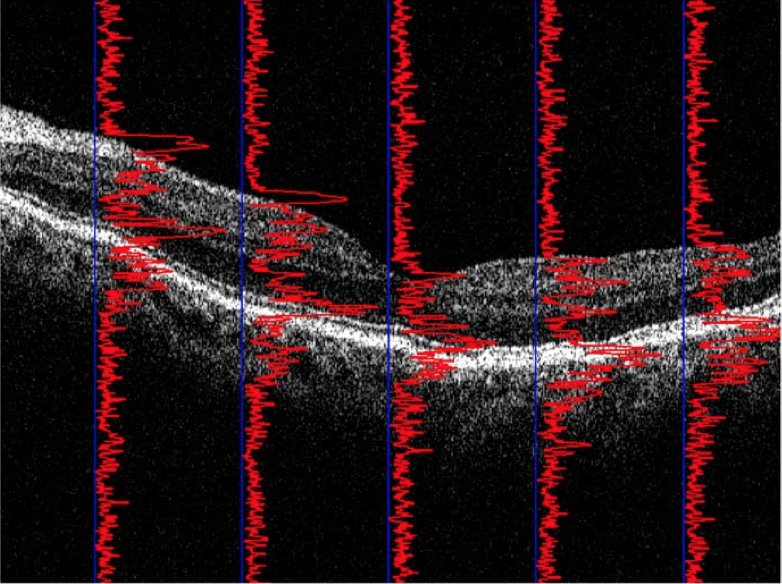
\includegraphics{figures/morgan_3}
\caption{A cross-sectional grey-scale image of the retina, built up from many A-scans which are illustrated as red plot lines. \cite{mbib_6} }
\label{fig:m_3}
\end{figure}


The above description is how Time-domain OCT utilizes low coherence interferometry.
The other option is having a fixed reference mirror and attaching a spectrometer to
the detection arm to record the spectral signal produced by the reflected
 “bursts” of light, which is known as Spectral-domain OCT.\cite{mbib_3} The next
section will go into more detail on the different imaging methodologies.

\section{Time-Domain and Spectral-Domain Optical Coherence Tomography}
Time-domain and Spectral-domain Optical Coherence Tomography differ in the way
the backscatter of the light from the super-luminescent diode from the retinal
tissues is analysed.  To briefly describe the differences between the two main
methods: TD-OCT resolves depth by measuring its flight time through the retina,
whereas SD-OCT uses a spectrometer to measure the difference in wavelength
between the light from the fixed reference arm and that of the light returning
from the retinal tissues to generate these cross-sectional images.\cite{mbib_7}

In both cases, the light wave travels through the retina as illustrated in \fref{fig:m_4} and
is reflected from each layer (detailed image of these layers can also be
found in \fref{fig:m_4} ) because the layers have different refractive indices.
Thus the backscatter of the light from deeper tissues can be differentiated from
backscatter returning from more superficial tissues because it takes longer for
the light to arrive at the sensor; a physical principle utilized in Time-domain OCT
imaging.\cite{mbib_4}

Time-domain OCT is when the reference mirror is mechanically moved to different
positions using the galvanic mirrors with freedoms in the x and y directions,
resulting in a time difference between the light from the reference arm and the
light returning from the retinal tissues.  These time differences depend on the
depth at which the light is backscattered from and can be used to reconstruct
retinal structure.  Since the speed at which the mirrors can be moved is limited
mechanically, only thousands of A-scans can be generated per second.” \cite{mbib_4}

\begin{figure}[htbp]
\centering
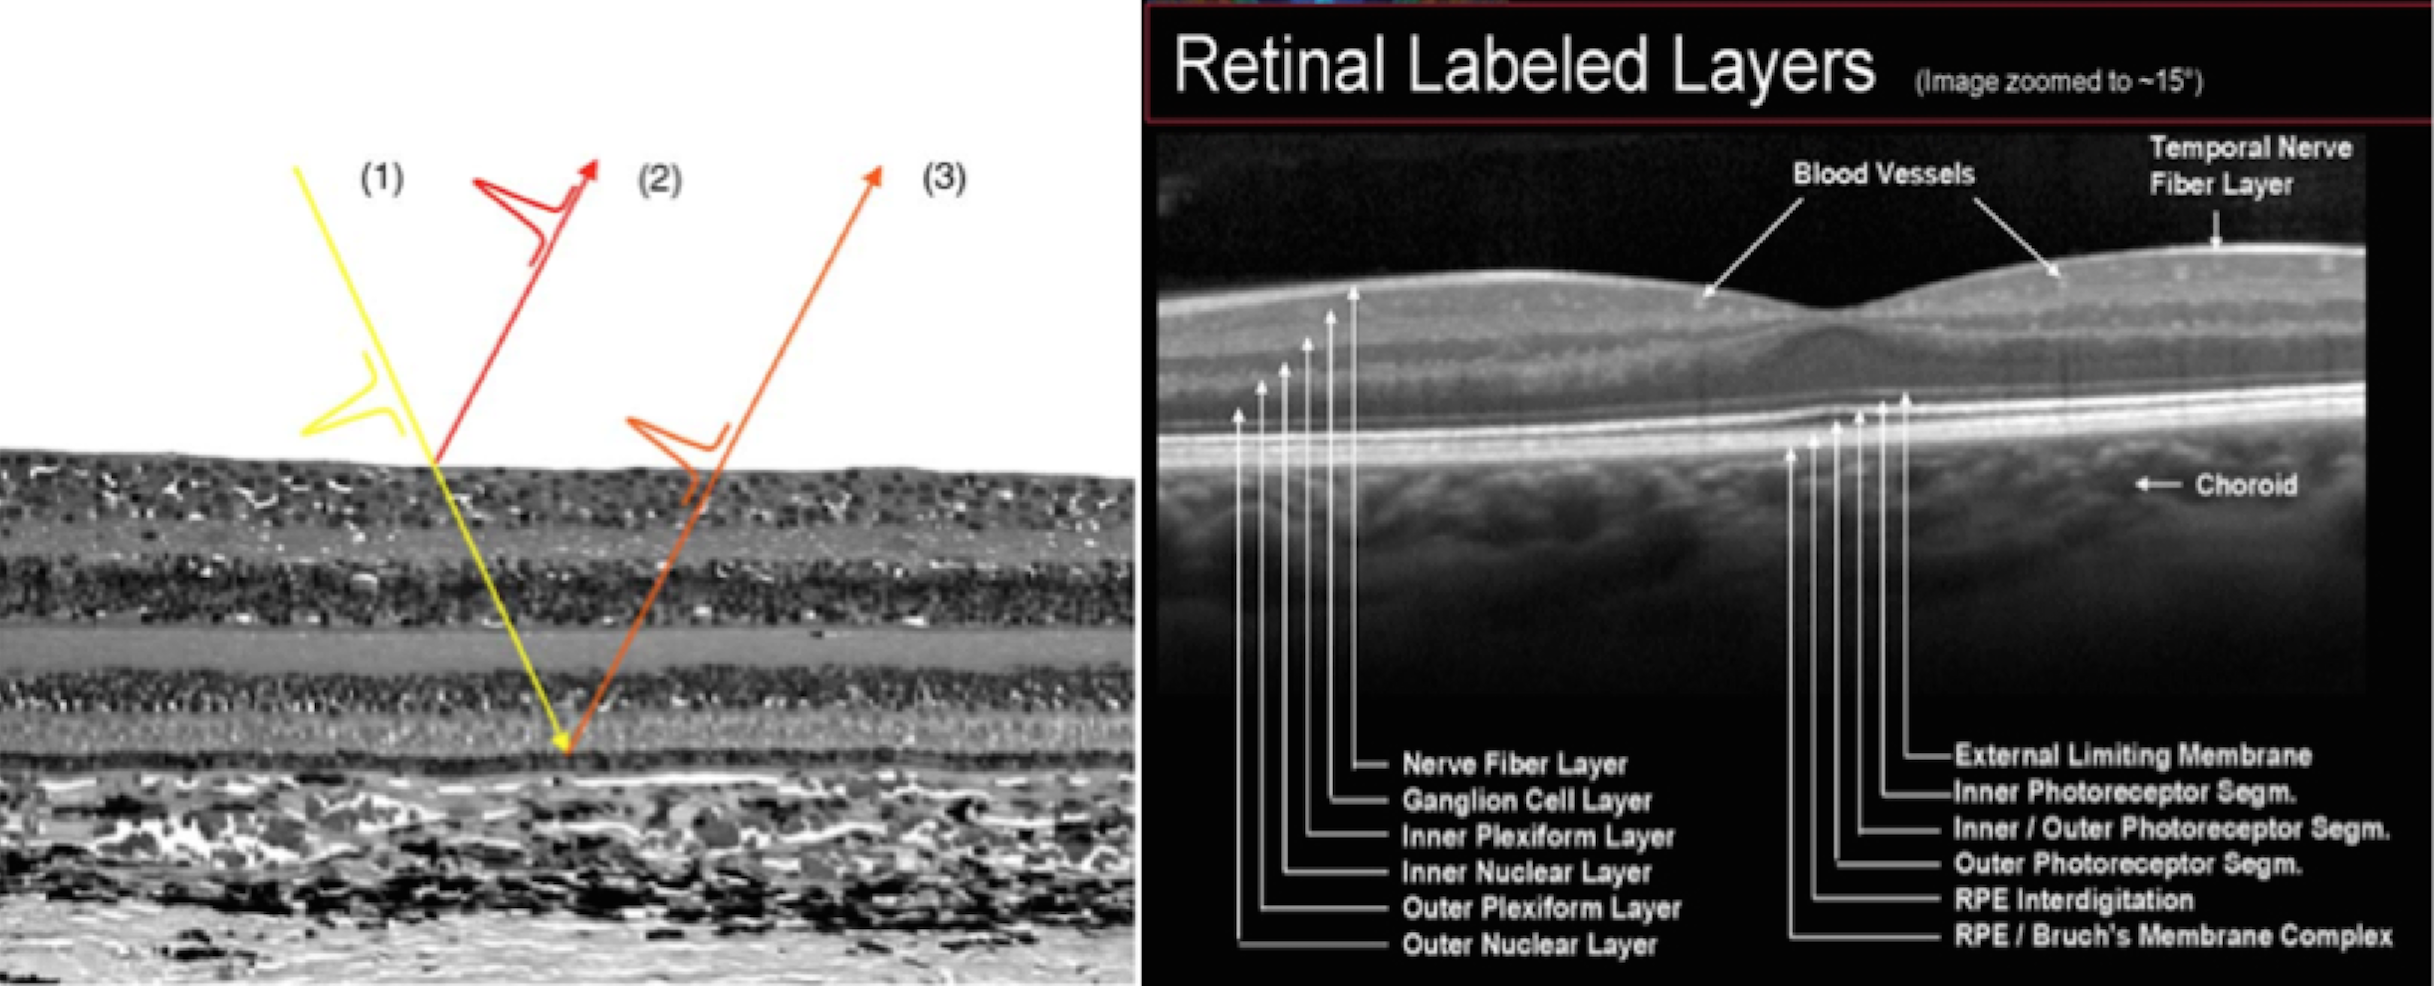
\includegraphics{figures/morgan_4}
\caption{(Left) "The optical coherence tomography beam is scanned across the retina (1).
The delay of a superficial reflection (2) is shorter than that of a deeper reflection (3)" (Right) A two dimensional black and white SD-OCT scan with an image zoom of 15$^\circ$.\cite{mbib_6}  This scan shows the retina with retinal
tissue layers labelled using arrows to give meaning to the image.\cite{mbib_8} }
\label{fig:m_4}
\end{figure}

Another physical principle that is utilized in Spectral-domain OCT imaging is the
fact that the reflected light will have a different spectral fingerprint than the
initial light sent into the eye which will return from the reference arm.  Instead
of continuously moving the reference arm, as in TD-OCT, the reference arm is kept
fixed.

The main difference between Fourier-domain and Spectral-domain OCT is that in
FD-OCT the SLD’s light is rapidly modulated over its centre wavelength providing
another tag to the light; whereas in SD-OCT a broadband light source is used,
and the signal from the interferometer is spectrally decomposed using a diffraction
grating and a CMOS (Complimentary Metal Oxide Semiconductor) or CCD (Charged Coupled Device) linear sensor.\cite{mbib_4}
Thus a spectrometer is used to detect the spectrum created by the backscatter to
produce an image of the retina.  Once the signal is obtained a Fourier transform
(a mathematical procedure which extracts the frequency spectrum of a signal) is
applied to the spectral signal to determine the depth of all resultant scatters from
the tissues at the x and y coordinates.\cite{mbib_4,mbib_9} SD-OCT technology
proves to be more advanced than original TD-OCT in that it provides greater
resolving power of the retinal layers, significantly higher scan density, and faster
data acquisition. \cite{mbib_2}

\section{Images}
A-scans and B-scans were mentioned previously at the end of the low
coherence interferometry section.  For many years two dimensional B-scans were
the highest achievable image possible because OCT technology could not take
images fast enough to acquire enough images to construct a three dimensional
image of the retina.  Due to patient comfort, and safety requirements limiting how
much light can be projected onto the retina, images can only be taken for 1-3 seconds. \cite{mbib_4} With the improvement of SD-OCT, hundreds of thousands
of A-scans can be taken a second as opposed to the 400 A-scans a second achieved by
commercially available TD-OCT machines; making three dimensional images of the retina
possible.\cite{mbib_4}  Three dimensional images are now widely used in the clinical
setting as a standard of care.  As the technology improves, increasing the number of
A-scans taken in a second, higher resolution can be achieved in 3-D image volumes.\cite{mbib_4}  \fref{fig:m_9} illustrates the difference between the two 
and three dimensional images.

\begin{figure}[htbp]
\centering
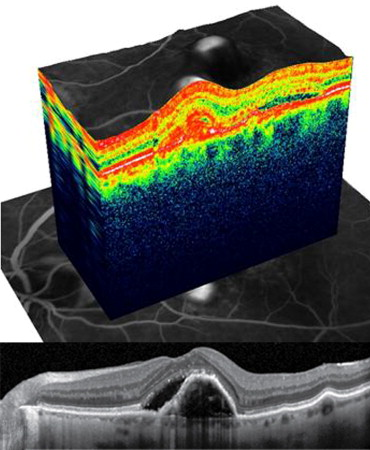
\includegraphics{figures/morgan_9}
\caption{ Overlay of the different retinal image scans using optical coherence tomography. The top image is a three dimensional image of the retinal with a fundus image below, and the bottom image is a two dimensional B-scan of the same retina which was used with a series of B-scans to produce the three dimensional image appearing above. \cite{mbib_13} }
\label{fig:m_9}
\end{figure}

The overall resolution of these images in the x and y directions is dependent on the
speed and quality of the galvanic mirrors used in TD-OCT.  In the z direction the
coherence of the light limits the resolution.  Both of these limitations were mentioned
previously in the section describing the methods of analysing the returning light
backscatter from the eye.

Ultimately OCT imaging technology is looking for a way to achieve isotropic images
of the retina, meaning the size of each element imaged is the same in all three
dimensions.  OCT devices commercially available currently can only achieve images
isotropic in the x-y plane, and have pixel volume sizes
of 30 × 30 × 2 $\mu m$. \cite{mbib_4}
This is because current OCT technology always has higher resolution of depth than
in the x-y plane. \cite{mbib_4}  Although a completely isotropic image is not possible
with current technology, there is an advantage to having “x−y isotropic imaging”.\cite{mbib_4} This method reduces the number of assumptions that 
have to be made when combining different retinal tissue sample
images, and allows the properties of the retina to be readily quantified for medical purposes.\cite{mbib_4} This helps ophthalmologists add more accurate images to the collection of information
making up retinal morphology.

Although the images are of high quality and resolution, the practitioner must consider
some other limitations.  For example corneal conditions such as dry eye, blinking, and
dilation of the eyes.  To tackle these limitations: dry eye can be addressed by applying
artificial tears to the patient’s eyes prior to the examination; blinking can be prevented
by shortening the scanning time and having the patient focus on the stimulus (which appears as a cross of green segments similar to that of a star); and in order to
achieve a larger scan of the retina, many practitioners dilate the patients eyes as
in many other retinal imaging examinations.\cite{mbib_4}

\section{Medical Applications of OCT}
OCT has many biomedical applications, however, the chief among them is retinal imaging and is particularly useful for monitoring, identifying, and quantitatively
assessing retinal diseases.\cite{mbib_9,mbib_4, mbib_5}  Before OCT there was
very little information in the database of retinal morphology.  With OCT imaging
this database has grown, providing a wealth of new information and has enabled
practitioners to closely  monitor retinal diseases and help guide them in the treatment
of patients with existing problems for therapeutic purposes.\cite{mbib_4}

OCT imaging currently used widely to determine the extent and amount of
retinal thickening to help guide these treatments prior to operation, as well as postoperative 
monitoring to ensure the patient is healing as expected.
This is done by imaging the thickness of the retinal tissue layers to find areas where a
retinal layer is thicker than the rest of that layer in the rest of the retina.  Retinal
layer thickness is the most common property currently utilized by medical professionals
in the tracking and diagnosing of retinal diseases, however, other properties can be looked
into such as analysing the images for textural properties in each of the layers, and quantifying
fluid parameters. \cite{mbib_4}

\subsection{Diabetic Macular Edema (DME)}
The most common application is in diabetic macular edema (DME). A patient with DME  leaks
fluid in the macula which in turn causes visual loss in said patient.  An original research
paper titled Early Treatment in Diabetic Retinopathy Study demonstrates that early treatment
of patients with DME with a focal laser can prevent further visual loss when targeting the
thickened areas of the retina. \cite{mbib_4}  This is done by analysing the thickness of the
retina and determining if there is an area of a retinal layer that is thicker than the rest.
An example of an OCT scan of someone with DME can be found in \fref{fig:m_5}.

\begin{figure}[htbp]
\centering
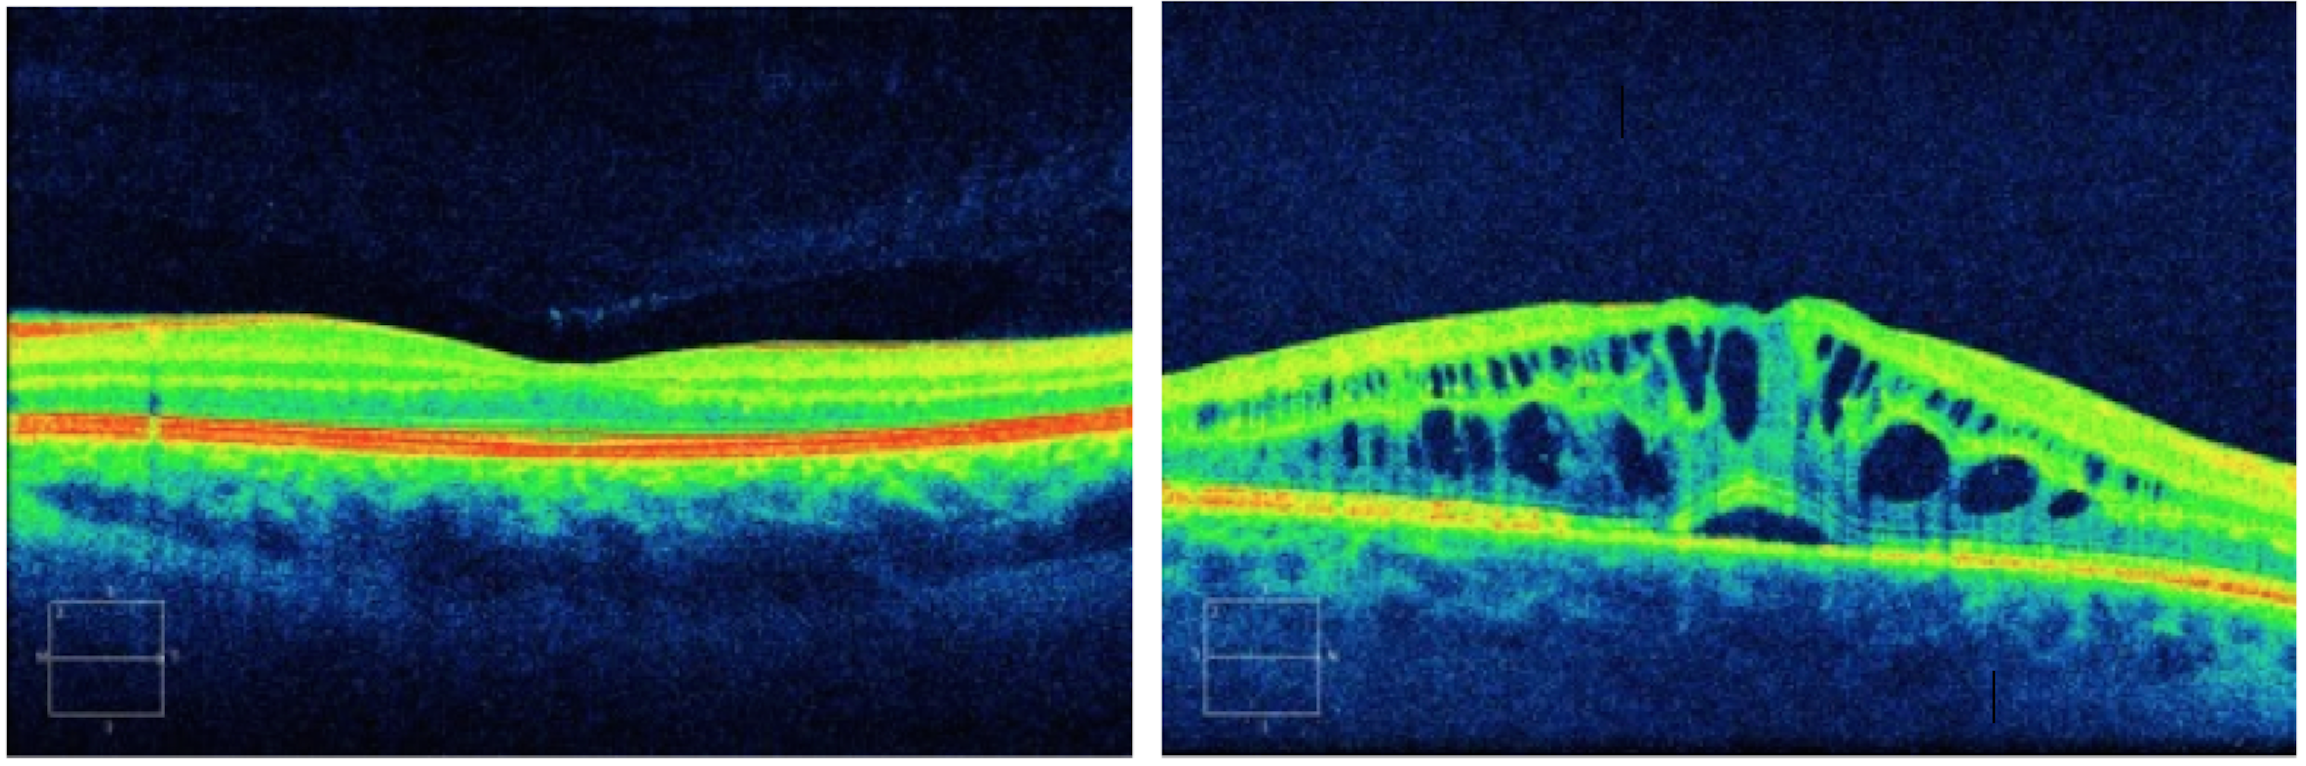
\includegraphics{figures/morgan_5}
\caption{Two images appear in this figure.  The left is an image demonstrating a patient with a normal retinal OCT scan in pseudo colours, while the left is that of a patient suffering from DME. \cite{mbib_10} }
\label{fig:m_5}
\end{figure}

\subsection{Glaucoma}
Glaucoma is a disease which causes gradual damage to the optic nerve.  
As mentioned in \cref{anatomy}, the result of this damage is visual field 
loss. \cite{mbib_6} If diagnosed early, this 
disease can be treated to reduce the risks of vision loss by using OCT 
images to observe thinning in the retinal nerve fiber layer and ganglion cell 
layer.  Both layers are extremely useful in the treatment and management 
of glaucoma as they serve as indicators of the extent of the optic nerve 
damage. \cite{mbib_4}
Since the optic nerve is where glaucoma manifests, the optic nerve head 
is another structure important to the study of glaucoma. \cite{mbib_4}
Along with thickness analysis, texture analysis can also be useful in the 
care for patients with glaucoma.  Texture analysis is possible by utilizing 
the local variations in brightness within one small area of an 
image. \cite{mbib_12} \Fref{fig:m_6} is an image of example optic nerve 
OCT image analysis and compares the different methods of analysing 
the images.

\begin{figure}[htbp]
\centering
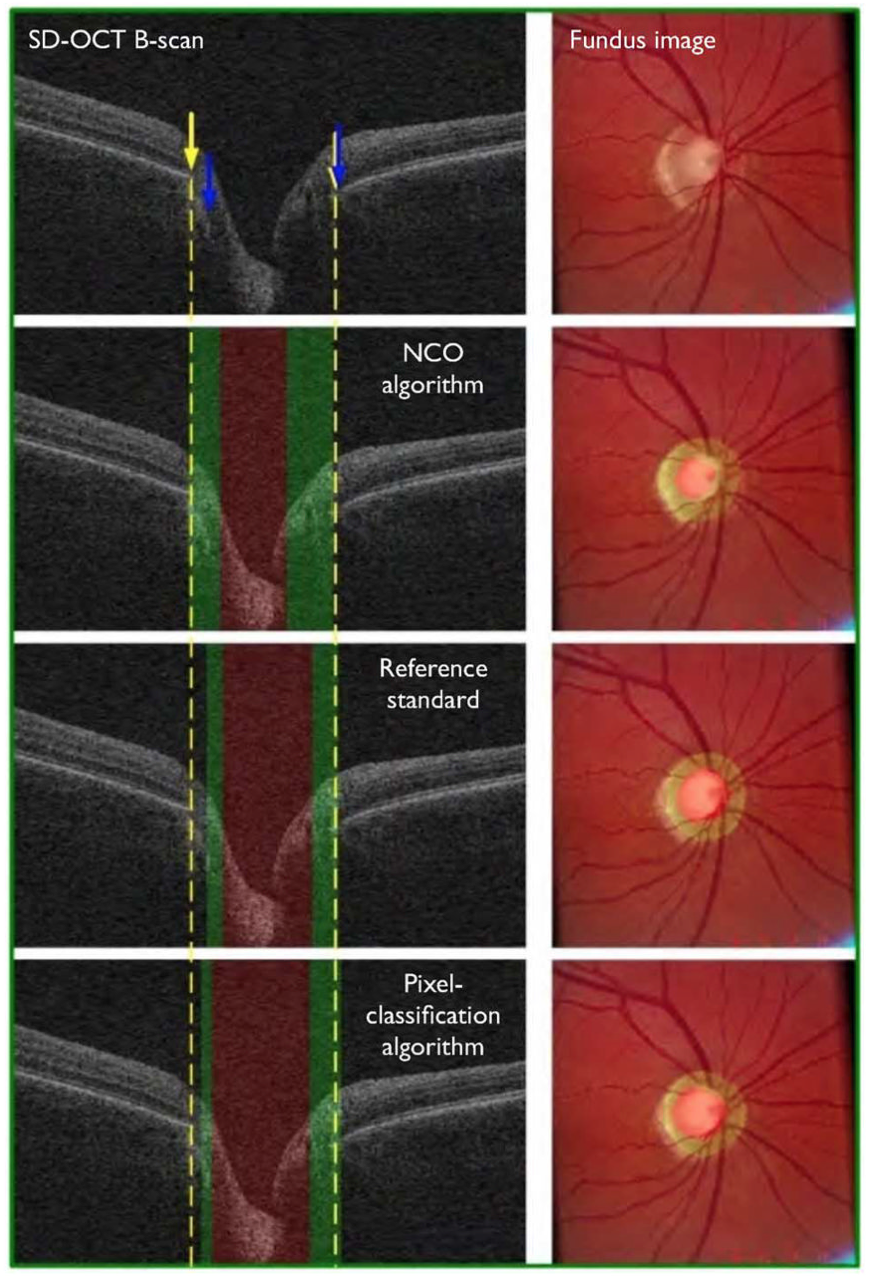
\includegraphics{figures/morgan_6}
\caption{This figure includes from top to bottom: a raw SD- OCT B-scan and corresponding
fundus image (top), structure-based (row 2), expert on fundus photography (row 3) and
pixel-classification-based (bottom) segmentations overlapping with raw SD-OCT and
corresponding fundus image.  From left to right: SD-OCT central B- scan (left) and
fundus image (right).  Yellow arrows indicate the position of the neural canal opening
(NCO) from algorithm (with dashed yellow line indicating projected NCO position).
Blue arrows indicate clinical disc margin from RS. Green and red colours indicate each
method’s projected rim and cup regions, respectively. \cite{mbib_4} }
\label{fig:m_6}
\end{figure}

\subsection{Symptomatic Exudate-Associated Derangements (SEADs)}
Another application of texture analysis is using textural properties along with
layer-based properties to detect retinal lesions in both two and three dimensional
OCT images. Out of all of the different types of lesions, symptomatic exudate-associated derangements (SEADs) are the prime interest of
experts assessing the severity of diseases such as age-related macular degeneration and diabetic macular edema.  SEADs are detected in a two step process when analysing OCT images.  First, possible candidates are identified in the OCT scans after the retinal layers are segmented (a process by which the different layers are separated from each other in the image) and the image is then flattened (when the curve of the layers due to the curve of the retina is flattened).  Once flattened, the area is then analysed to determine whether or not the candidate is a SEAD or not. 
\cite{mbib_4} Examples of these can be found in \fref{fig:m_7}

\begin{figure}[htbp]
\centering
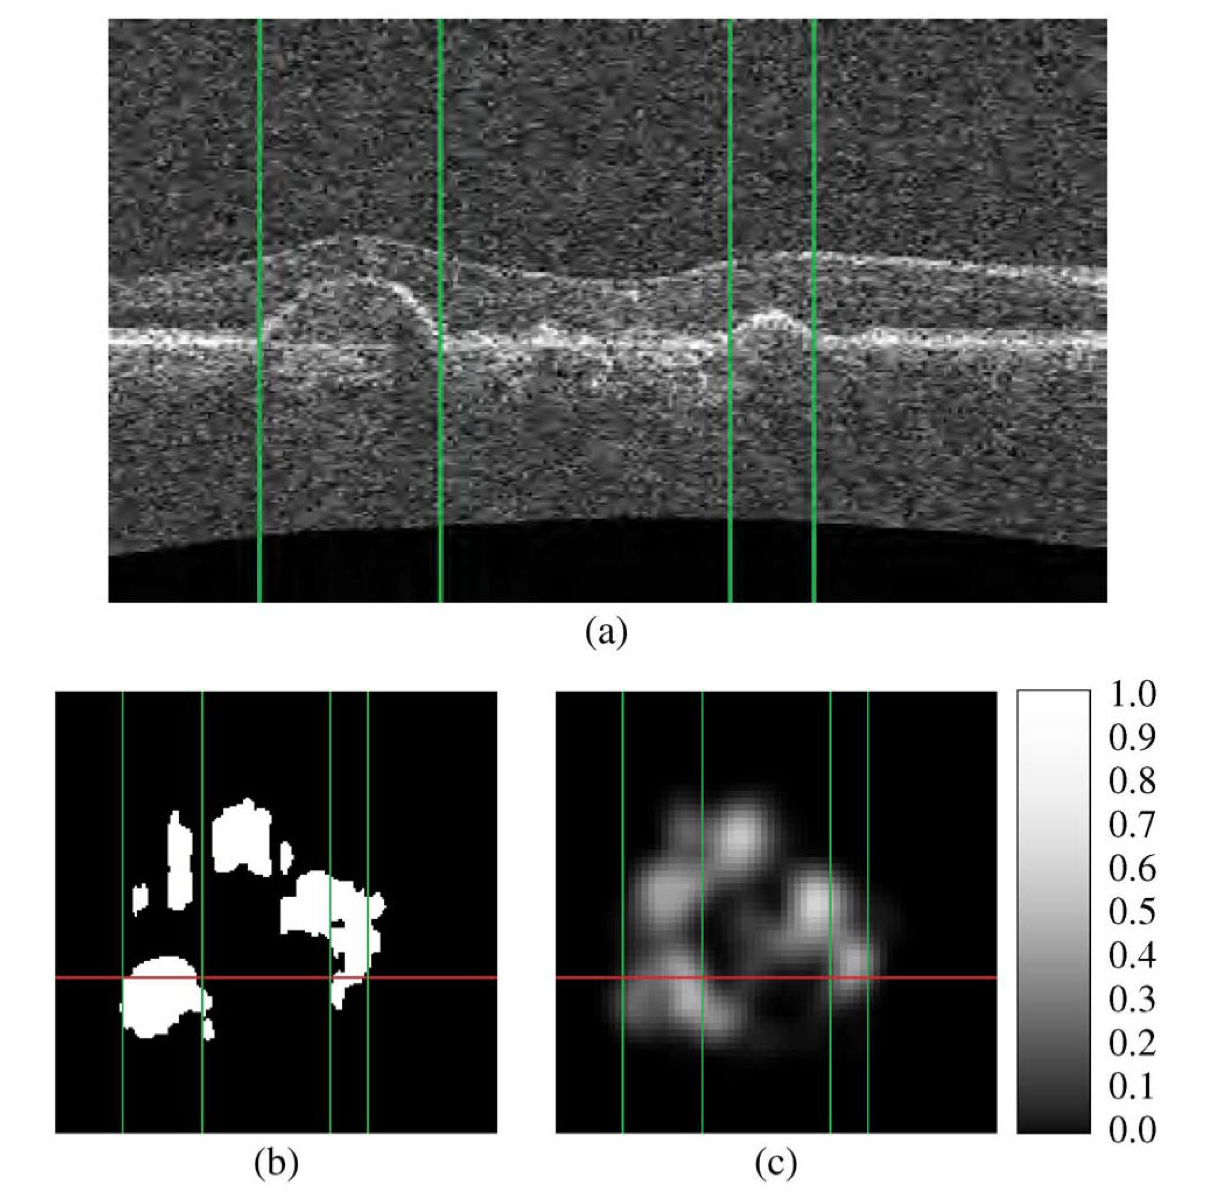
\includegraphics{figures/morgan_7}
\caption{SEAD footprint detection: (a) is an x-z slice running through the SEADs in SD-OCT volume; (b) and (c) are SEAD probability maps in x-y generated automatically using expert standards.  Note the probability scale in panel (c). Projection of the x − z slice in x − y plane is represented by a vertical line in (b) and (c). The location of the SEADs which are visible in panel (a), are indicated by vertical lines in each panel. \cite{mbib_4} }
\label{fig:m_7}
\end{figure}

\subsection{Choroidal Neovascularization}
Choroidal neovascularization is another blinding disease clinically known as the wet form of macular degeneration due to age.  The main indicators of this disease are outer and sub-retinal fluid. \cite{mbib_4}  By using OCT imaging to quantify fluid parameters and affected retinal tissues in patients with this disease, proper treatment can be applied.\cite{mbib_4} \fref{fig:m_8} is contains an OCT scan of someone suffering from choroidal neovascularization.

\begin{figure}[htbp]
\centering
\includegraphics{figures/morgan_8}
\caption{ Optical coherence tomography images show a sub-foveal choroidal neovascular membrane associated with sub-retinal fluid and cystoid macular edema at baseline (first row) and below are one month follow-up optical coherence tomography scans which show the disappearance of cystoid edema and complete resolution of sub-retinal fluid post treatment. \cite{mbib_11} }
\label{fig:m_8}
\end{figure}

\section{Further Improvements}
The current state of OCT technology can already achieve much better images 
of the retina than the
original technology developed in 1991.  Previously unachievable
capabilities of these machines are now clinically standard practice in the
medical diagnosis of several retinal diseases.  Although these improvements
are highly effective in improving the technology for retinal imaging, further
research can be done to obtain images of deeper structures within the eye such
as the choroidal vessels, which are a structure in the optic nerve and
relevant to the study of damage caused by glaucoma. \cite{mbib_4}  Current
commercially available
machines use wavelengths around 840$\mu m$ and only allow medical professionals
to image the retina.  Longer wavelengths around 1000-1300 $\mu m$ would enable
the OCT imaging light to penetrate deeper into the tissue and image deeper
structures such as choroidal vessels. \cite{mbib_4}

% Author: Eskil Joergensen
% Tex Author: Magdalen Berns
% Formatting: Magdalen Berns

\chapter{Future Research of Retinal Imaging and Analysis}

\label{future_research}
\lhead{\emph{Future Research in Retinal Imaging}}
\section{Future Research in Retinal Imaging}
\label{future}

\section{Cheap Retinal Scanners for global accessibility}

The development of an economic and accurate system for an early
glaucoma and diabetic retinopathy. As the most common roots of
blindness, an early detection of both conditions are vital for
curing the diseases. The damages done at the point of discovery
are non-reversible. The development of an easy-to-use cost-effective
apparatus would mean patients can be checked and hence be treated
more easily.

With rapidly growing number of patients due to lifestyle-illnesses,
including a diabetes (type II), health institutions would be able
to save both capacity and resources if such tools were readily
accessible. An early diagnosis of diabetic retinopathy reduces
the risk of blindness of 50\%.\cite{}

Today, besides the equipment, the study of retinal images in medicine
is expensive and time consuming as an ophthalmologist has to analyse
the images in order to make a diagnosis. This is a process that can
be automated by computers.  In 1996 a correct identification rate of
88.9\%
was achieved by automated computer-analysis, which means that the
retinal images can be taken and analysed automatically. The potential
patients can then be filtered and referred to a health professional
to receive proper treatment.\cite{}

( With an increasing number of connections associating the health
of the retina with modern lifestyle-illnesses, being able to produce
cheap and reliable retinal imagery apparatus is an important step for
early identification and swift treatment of such deceases. ) With
recent advances in the state of wearable technology, personal devices
can now monitoring heart rates, sleeping cycles and hydration levels.
Having personal devices that are able to monitor the stress (and
general health condition) of the eye would be the idea solution.
Currently there are composite devices that are able to take "simple"
images of the retina\cite{}.
 
\section{Blue light hazard}

The effect of blue light LED on macular degeneration and retinal
damage. With fast-growing use of LED devices and energy-efficient
light bulbs, with a peak light-wavelength in the blue light region,
can cause increased oxidative stress on the retinal tissue.\cite{}
A chronic exposure to blue light can result in induced photochemical
deterioration of the retina, which has the effect of accelerating the
biological ageing. [Behar-Cohen F, Martinsons C, Vienot F, Zissis G,
BarlierSalsi A, Cesarini JP, et al. 2011. Light-emitting diodes (LED)
for domestic lighting: any risks for the eye?\cite{}

As everyday use of blue-intensive light sources is relatively new,
the long-term effects can be serious macular degeneration. Hence the
development of retinal imaging techniques are important in maintaining
the study of these trends and also better understanding the biological
effects on the retina.
 
Normal white light contains a wide distribution of "all" colour
wavelengths. Waves of different wavelength are either absorbed or
transmitted by the different sections of the eye. As a result,
being exposed to natural sunlight means that the different sections
of the eye are all used. By introducing a narrow range of light waves
means that some parts of the eye will be used more than others. In the
case of blue-intensive light waves, those are all absorbed by the retina
alone, as can be seen in the table [Light-emitting diodes (LED) for
domestic lighting: Any risks for the eye?\cite{}

\section{Multimodality}

Multimodality imaging is becoming increasingly common in
ophthalmology. For image information from multiple modalities
to be usable in mutual context, images must be registered so
that the independent information that was acquired by different
methods can be concatenated and form a multimodality description
vector. Thus, because of its importance in enabling multimodal
analysis, retinal image registration reflects another active
area of research. The several clinically used methods to image
the retina were introduced above and include fundus photography,
scanning laser ophthalmoscopy, fluorescence imaging, and OCT.
Additional retinal imaging techniques such as hyper-spectral imaging,
oxymetry, and adaptive optics SLO will bring higher resolution.

To achieve a comprehensive description of retinal morphology
and eventually function, diverse retinal images acquired by different
or the same modalities at different time instants must be mutually
registered to spatially combine all available local information.
The following sections provide a brief overview of fundus photography
and OCT registration approaches in both two and three dimensions.
Registration of retinal images from other existing and future imaging
devices can be performed in a similar or generally identical manner.

\section{Security}

Using the unique biometrics of the eye (iris and retina) one can set up
certain system to recognise these patterns. For security purposes the use
of the unique retina pattern has many advantages and applications. The
pattern of the retina, which maps the locations of veins, arteries the
macula and the optic nerve in the eye, has a much more complex pattern
than the normally used fingerprint or iris scan.\cite{} Personal
iris patterns and fingerprints are accessible to others, this means
they are more easily copied. Where a thumb can be amputated and still
be used in a scanner, the blood vessels mapping across the retina would
contract so quickly that having someones "amputated" eye would not help
in tricking a retina recognition scanner. As a result using retinal
imaging as the ultimate personal identification is possible.

In terms of consistency a retina scan has an error rate of 1 in 10 000 000,
whereas the error of a fingerprint scan can be as high as 1 in 500.\cite{}

\chapter{Conclusion}

\label{conclusion}
\lhead{\emph{Conclusion}}

This report has sought to provide an extensive investigation
into the technology that underpins retinal imaging, from the
early origins of ophthalmoscopy in the 19th century, through the 
currently used fundus cameras, cSLOs and OCT machines and up 
to the most recent advancements in imaging technology utilizing 
adaptive optics and two-photon microscopy. Before this was done, 
a detailed look into the eye and it?s dysfunction, pathology, and 
injuries was carried out to provide the necessary background for 
retinal imaging research.

Initial retinal imaging devices were able to document a wide array 
of common pathology; with glaucoma, diabetic retinopathy and macular 
edema all observable using primitive fundus photography and 
ophthalmoscopy. The ability of the early machines to detect 
disease once it had manifested to a sight threatening level provided 
useful information to ophthalmologists, however, it was of little help 
in preventing vision loss. 

With improvements in image resolution in fundus cameras came 
the ability of devices to detect symptoms of disease development, 
resulting in the onset of early detection screening programmes. 
Following this, practitioners became concerned with imaging 
wider visual fields and achieving greater depth penetration into 
the retinal tissue, to learn more about the how certain diseases 
manifest themselves across the retina. This resulted in the 
development of the cSLO and the OCT, which widened the scope 
of the visible retina by accessing the peripheral retina and obtaining 
higher resolution within retinal layers for closer study.  Yet again 
expanding the diagnostic capability of eye-care professionals. 

These devices have been key in the progression of retinal disease 
study and have encouraged further technological developments. 
These developments aim to widen the scope of current machines 
and bring them to areas of the world that do not have adequate 
infrastructure to support widespread use. With new equipment and 
new diagnostic systems, retinal imaging technology will be able to 
provide a valuable clinical tool to help patients preserve their vision 
in the developing world by making them affordable and easy to use.
 
Increasing rates of diabetes and a globally aging population are 
challenges that have to be met with the development of innovative 
methods. Specialists therefore must continue to develop high 
quality imaging devices to respond to global healthcare demands. 

\chapter{Glossary}

\label{glossary}
\lhead{\emph{Glossary}}

\glsaddall

\printnoidxglossaries


%-------------------------------------------------------------------------------
% CONTENT - APPENDICES
%-------------------------------------------------------------------------------
\addtocontents{toc}{\vspace{2em}}

%\appendix

%\input{Appendices/AppendixA}

\addtocontents{toc}{\vspace{2em}}



\backmatter



%-------------------------------------------------------------------------------
% BIBLIOGRAPHY
%-------------------------------------------------------------------------------

\label{Bibliography}

\lhead{\emph{Bibliography}}

\bibliographystyle{unsrt}

\bibliography{bibliography}

\end{document}
